\documentclass[onecolumn,10pt]{article}
\linespread{1.3}
\usepackage[margin=2cm]{geometry}

\usepackage[utf8]{inputenc}
\usepackage[spanish]{babel}
\usepackage{tikz}
\usepackage{paralist}
\usepackage{subcaption} \usepackage{graphicx}
\usepackage{amsmath} \usepackage{amssymb}
\usepackage{xcolor}
\usepackage{listings}

\usepackage{amsmath}
\usepackage{algorithm}
\usepackage[noend]{algpseudocode}

\lstset{language=C}
\bibliographystyle{apsrev4-1}

\graphicspath{{./fig/}}

\newcommand{\IDT}{\texttt{IDT}}
\newcommand{\MMU}{\texttt{MMU}}
\newcommand{\GDT}{\texttt{GDT}}
\newcommand{\TSS}{\texttt{TSS}}
\newcommand{\PD}{\texttt{PD}}

\begin{document} 

\title{Trabajo Práctico 2: Redes Neuronales Artificiales}

\author{L. Alvarez, P. Bordon y D. Santos}

\date{\today}

%\begin{abstract}
%\end{abstract}

\maketitle


\newpage

\tableofcontents

\newpage

\par Se cuenta con documentos de descripción de empresas. Dichos documentos se encuentran preprocesados, de manera tal que se tiene un dataset que especifica qué cantidad de veces aparece cada palabra en cada documento. Este formato es conocido como Bolsa de Palabras (Bag-Of-Words). El problema a resolver será diseñar y entrenar una red neuronal mediante métodos de aprendizaje hebbiano no supervisado para que pueda clasificar automáticamente los documentos según categoría. También se busca que esta red pueda generalizar corréctamente y responda de manera certera a nuevos documentos.


\section{Ejercicio 1: Reducción de dimensiones}

\subsection{Introducción}

\par Para el primer ejercicio, queremos reducir la dimensionalidad de la entrada, debido a que es muy grande, a 3 valores. Para esto vamos a diseñar una red neuronal y la entrenaremos mediante aprendizaje hebbiano no supervisado aplicando la regla de oja y la regla de sanger. Luego analizaremos y compararemos sus resultados.

\subsection{Análisis de la Red}

\par En un comienzo, trabajamos con una red que contaba con 10 o 15 neuronas de salida para no reducir drásticamente su dimensión. Al final el entrenamiento, reducíamos la salida a 3 valores y obteníamos lo buscado. Luego de varias pruebas y cambios determinamos que no ganábamos nada tomando esta determinación, por el contrario, se áumentaba la complejidad del algoritmo y se perdía tiempo revisando la ortogonalidad de las 10 columnas de la matriz de pesos, mientras que los resultados obtenidos no eran mejores. Por esto se determinó manejar desde un inicio 3 dimensiones de salida.

\par Vale aclarar que las reglas de oja y sanger son formas de calcular el cambio que se debe hacer a la matriz de pesos para entrenarla. Por esto, ambos modelos son iguales, solo que se aplican distintos cálculos para cada tipo de regla.

\subsection{Procesamiento de Datos}

\par Sabemos que los valores de entrada son enteros positivos, ya que determinan la cantidad de apariciones de una palabra en un texto. Y al estar la entrada preprocesada y sin las palabras mas comunes (con mas apariciones), los valores de entrada se encuentran acotados. Podríamos no haber implementado ningún tipo de preprocesamiento, pero preferimos estandarizar la entrada, de manera que los atributos presenten media cero y varianza uno, moviendose en un rango de valores similar.


\subsection{Experimentación y Resultados}

\par Habiendo fijado el número de neuronas de salida a tres unidades, pasamos a implementar los dos algoritmos propuestos. En primera instancia trabajamos en una fase de entrenamiento, donde el parámetro de interés a optimizar es el coeficiente de aprendizaje, que bien puede ser función del número de época. Tanto la condición de ortonormalidad( $|| W^T \cdot W - I || = 0$) como la subsiguiente validación son las herramientas para determinar su valor óptimo. Comenzamos con un coeficiente de aprendizaje constante, siguiendo con funciones del tipo $\frac{1}{epoca^{\alpha}}$, con alfa entre 0 y 1. Probando estas distintas opciones encontramos que si bien no existían diferencias significativas, un coeficiente del tipo $\frac{1}{epoca^{\frac{1}{2}}}$ presentaba los mejores resultados.

\subsubsection{Algoritmo de Oja}

\par A continuación se pueden observar los resultados obtenidos utilizando el algoritmo de Oja separando el set de datos de entrada en 70\% - 30\%, para el coeficiente de aprendizaje adaptativo propuesto. Las figuras \ref{fig:  ej1_oja_3d_1} y \ref{fig: ej1_oja_3d_2} presentan los datos en el espacio 3d de salida obtenido por el algoritmo. Las figuras \ref{fig: ej1_oja_3d_1_train} y \ref{fig: ej1_oja_3d_2_train} corresponden a datos de entrenamiento, mientras que las figuras \ref{fig: ej1_oja_3d_1_valid} y \ref{fig: ej1_oja_3d_2_valid} corresponden a datos de validación. 

\begin{figure}[H]
        \begin{subfigure}[b]{0.5\textwidth}
                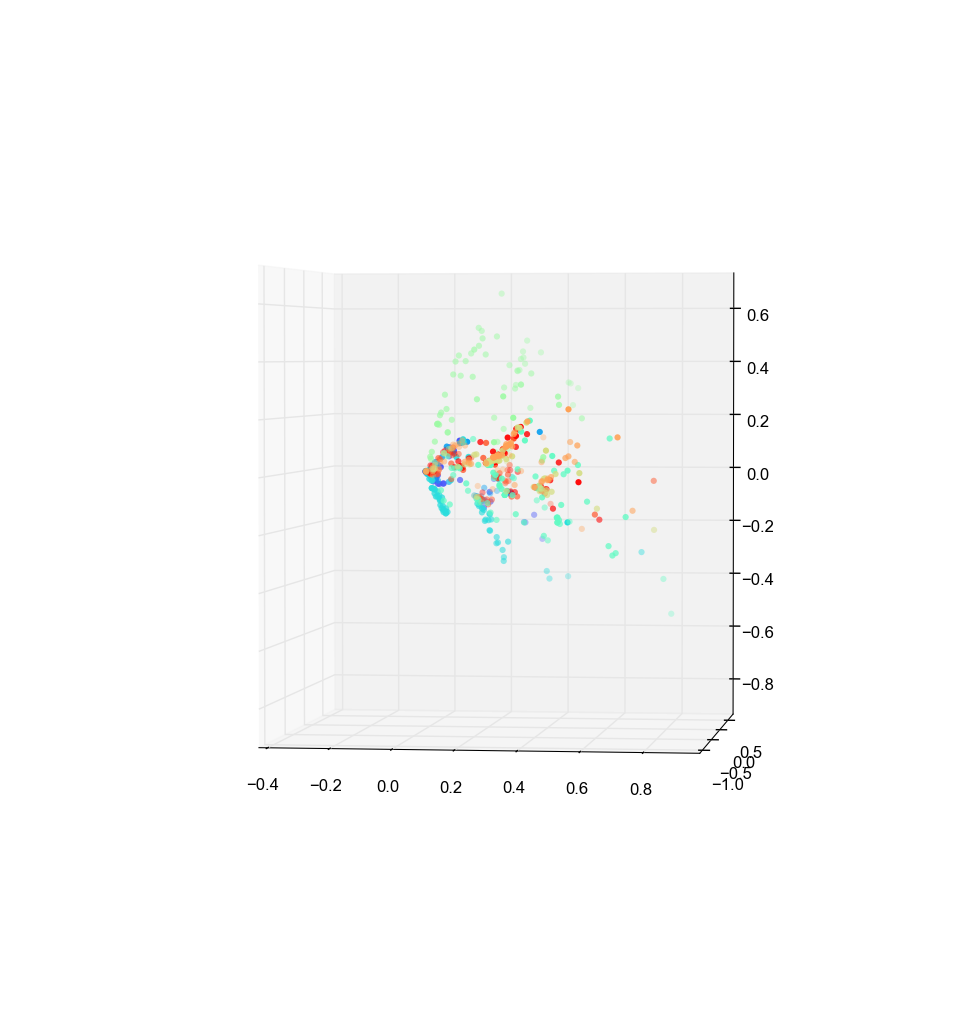
\includegraphics[width=\linewidth]{secciones/graficos/oja/1_train.png}
                \caption{Entrenamiento}
                \label{fig: ej1_oja_3d_1_train}
        \end{subfigure}%
        \begin{subfigure}[b]{0.5\textwidth}
                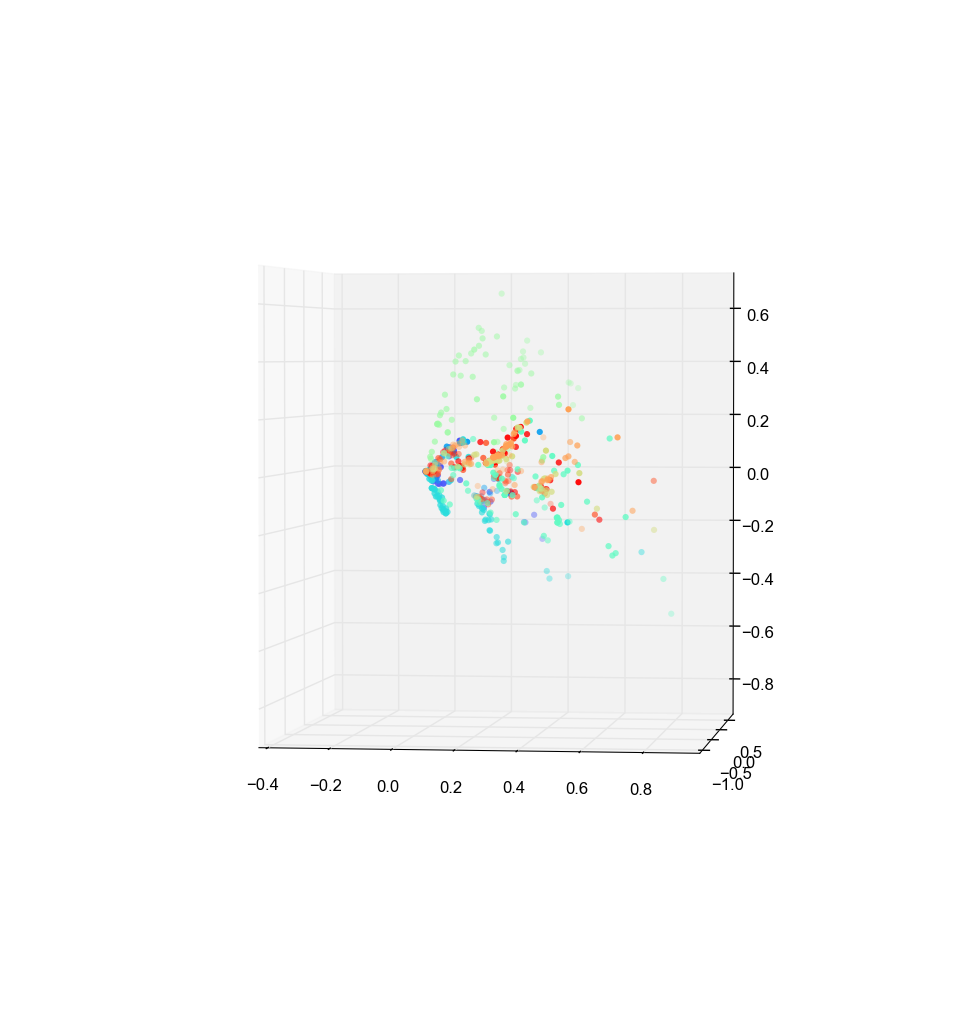
\includegraphics[width=\linewidth]{secciones/graficos/oja/1_train.png}
                \caption{Validacion}
                \label{fig: ej1_oja_3d_1_valid}
        \end{subfigure}
        \caption{Vista 1 en 3d de resultados de validación y entrenamiento}
        \label{fig: ej1_oja_3d_1}
\end{figure}

\begin{figure}[H]
        \begin{subfigure}[b]{0.5\textwidth}
                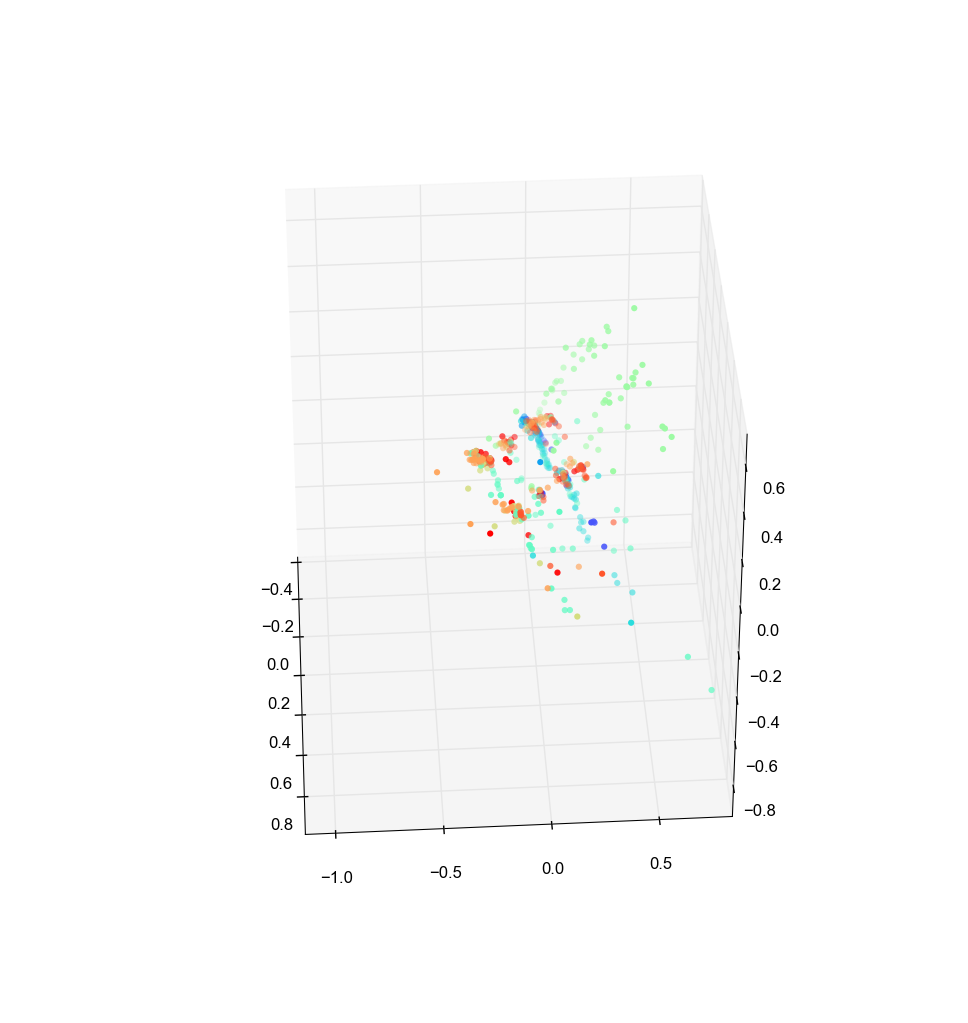
\includegraphics[width=\linewidth]{secciones/graficos/oja/2_train.png}
                \caption{Entrenamiento}
                \label{fig: ej1_oja_3d_2_train}
        \end{subfigure}%
        \begin{subfigure}[b]{0.5\textwidth}
                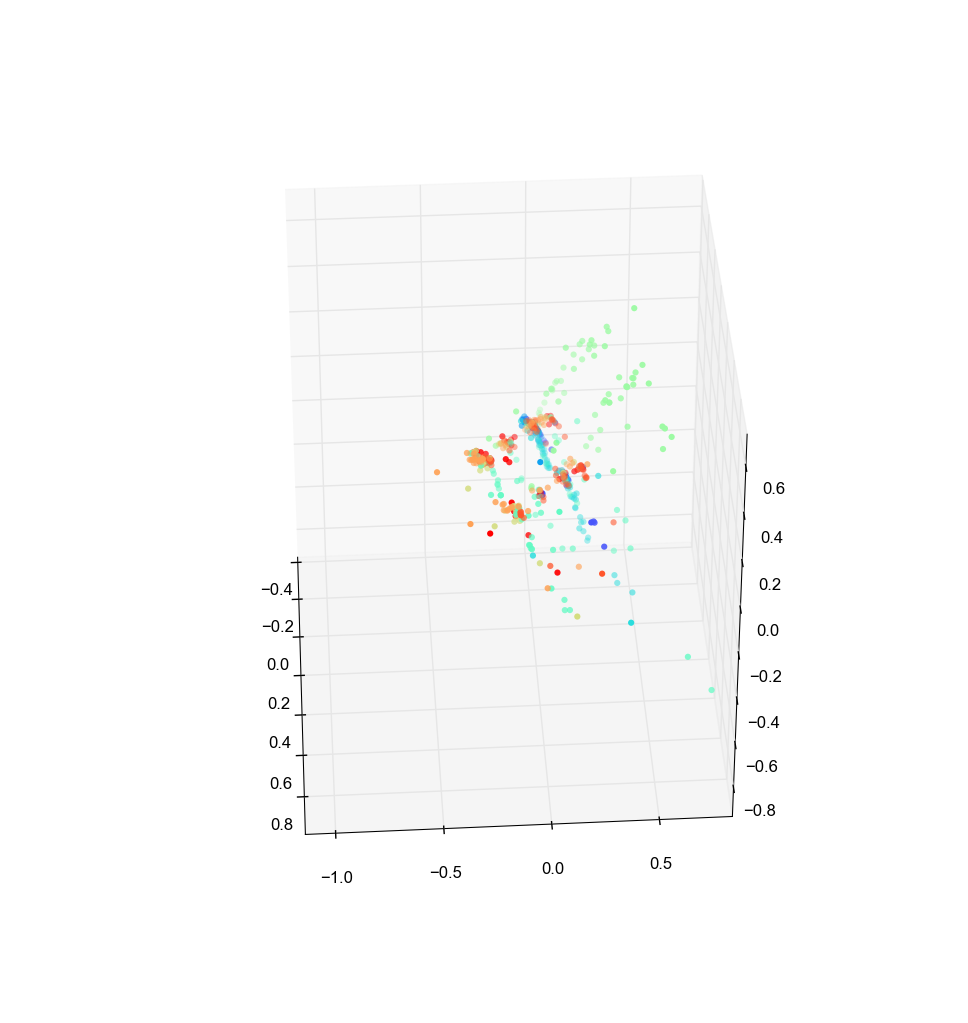
\includegraphics[width=\linewidth]{secciones/graficos/oja/2_train.png}
                \caption{Validacion}
                \label{fig: ej1_oja_3d_2_valid}
        \end{subfigure}
        \caption{Vista 2 en 3d de resultados de validación y entrenamiento}
        \label{fig: ej1_oja_3d_2}
\end{figure}


\par Se puede observar que la validación es consistente con la clasificación obtenida en la etapa de entrenamiento, dando cuenta de la validez del procedimiento realizado. También se puede observar en el gráfico claramente la separación entre dos de las categorías, la verde y azul, cosa que no ocurre para las categorías restantes. Para poder discriminar sobre estas últimas realizamos graficos 2d (figura \ref{fig: ej1_oja_ejes_train}), proyectando el gráfico 3d sobre tres planos distintos, tanto para los datos de entrenamiento \ref{fig: ej1_oja_ejes_train}  como para los de validación \ref{fig: ej1_oja_ejes_valid}.

\begin{figure}[H]
        \begin{subfigure}[b]{0.33\textwidth}
                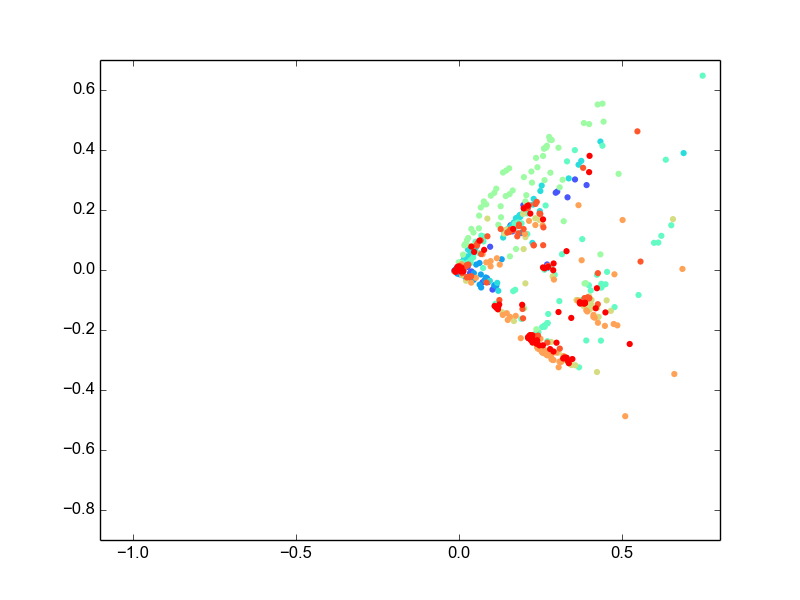
\includegraphics[width=\linewidth]{secciones/graficos/oja/eje1_train.png}
                \caption{Corte 1}
                \label{fig: ej1_oja_eje_1_train}
        \end{subfigure}
        \begin{subfigure}[b]{0.33\textwidth}
                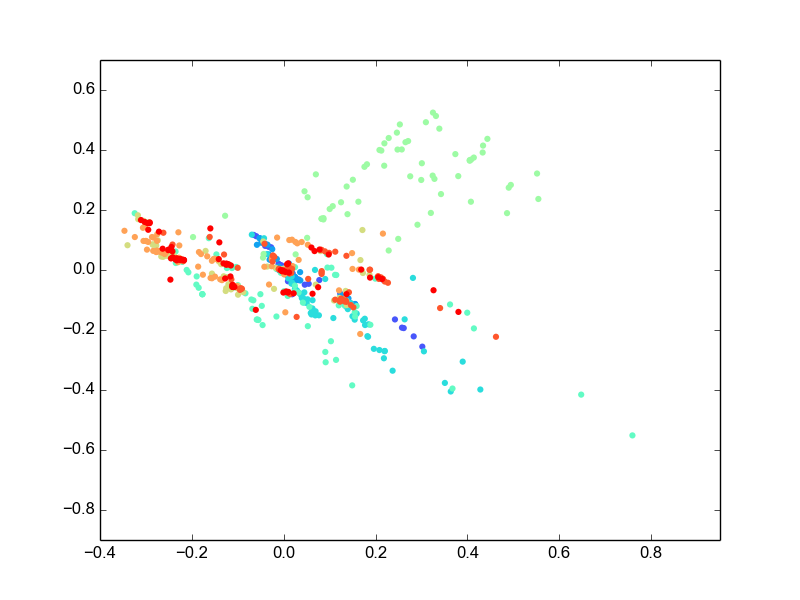
\includegraphics[width=\linewidth]{secciones/graficos/oja/eje2_train.png}
                \caption{Corte 2}
                \label{fig: ej1_oja_eje_2_train}
        \end{subfigure}
        \begin{subfigure}[b]{0.33\textwidth}
                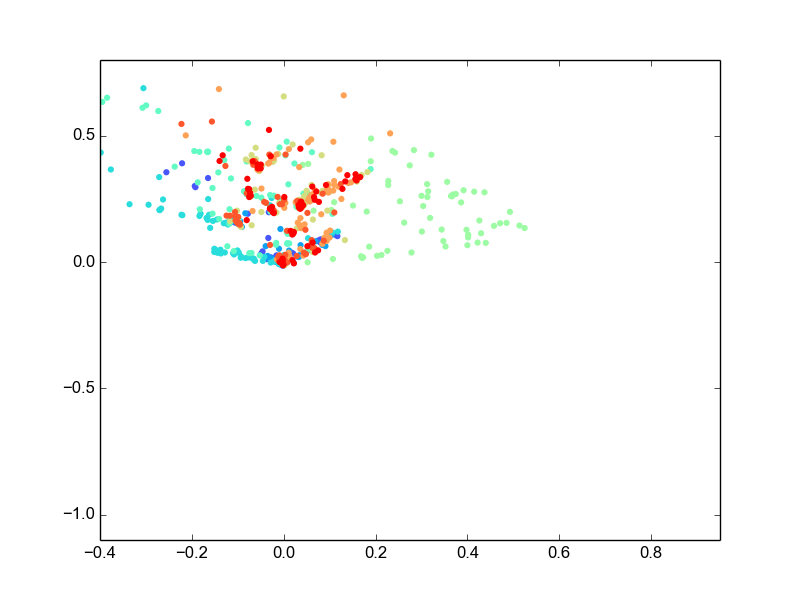
\includegraphics[width=\linewidth]{secciones/graficos/oja/eje3_train.png}
                \caption{Corte 3}
                \label{fig: ej1_oja_eje_3_train}
        \end{subfigure}
        \caption{Cortes del gráfico de los datos de entrenamiento}
        \label{fig: ej1_oja_ejes_train}
\end{figure}

\begin{figure}[H]
        \begin{subfigure}[b]{0.33\textwidth}
                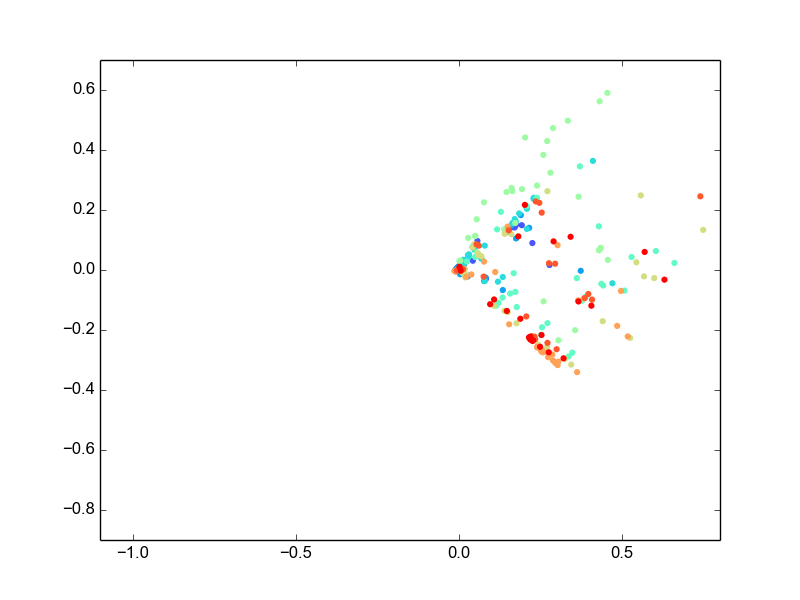
\includegraphics[width=\linewidth]{secciones/graficos/oja/eje1_valid.png}
                \caption{Corte 1}
                \label{fig: ej1_oja_eje_1_valid}
        \end{subfigure}
        \begin{subfigure}[b]{0.33\textwidth}
                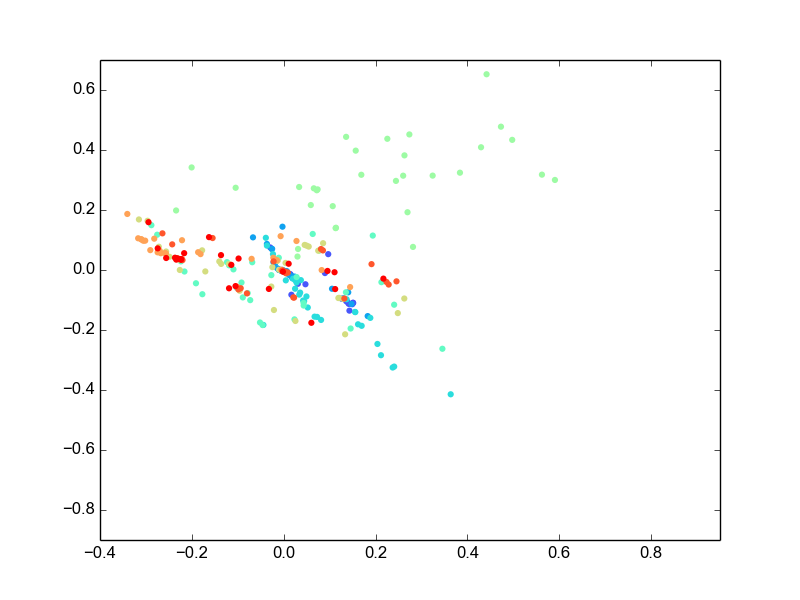
\includegraphics[width=\linewidth]{secciones/graficos/oja/eje2_valid.png}
                \caption{Corte 2}
                \label{fig: ej1_oja_eje_2_valid}
        \end{subfigure}
        \begin{subfigure}[b]{0.33\textwidth}
                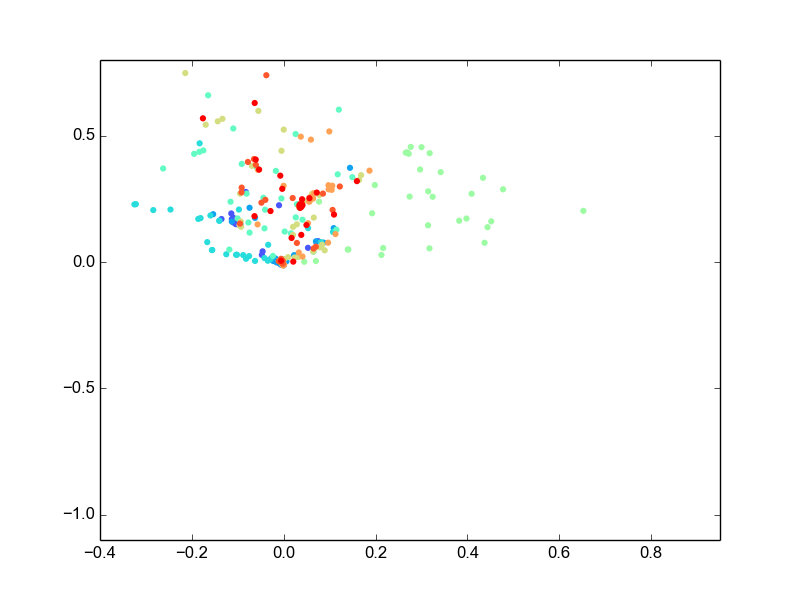
\includegraphics[width=\linewidth]{secciones/graficos/oja/eje3_valid.png}
                \caption{Corte 3}
                \label{fig: ej1_oja_eje_3_valid}
        \end{subfigure}
        \caption{Cortes del gráfico de los datos de validación}
        \label{fig: ej1_oja_ejes_valid}
\end{figure}


\par Estos gráficos permiten observar mejor las similitudes entre los resultados obtenidos con los datos de entrenamiento y los obtenidos con los datos de validación. No se distinguen resultados tan errado como para ser detectados a simple vista. Esto nos deja la impresión de que, a pesar de que las categorías no se separen y agrupen como esperábamos, la red generaliza bastante bien y es consistente en cuanto a la ubicación de las categorías.

\par A continuación realizamos un gráfico 3D para cada categoría en la etapa de entrenamiento, con la finalidad de poder observar su distribución individualmente, ya que en las figuras \ref{ej1_oja_ejes_train} se encuentran algo superpuestas. Los resultados se observan en las figuras \ref{fig: ej1_oja_categorias}.

\begin{figure}[H]
        \begin{subfigure}[b]{0.33\textwidth}
                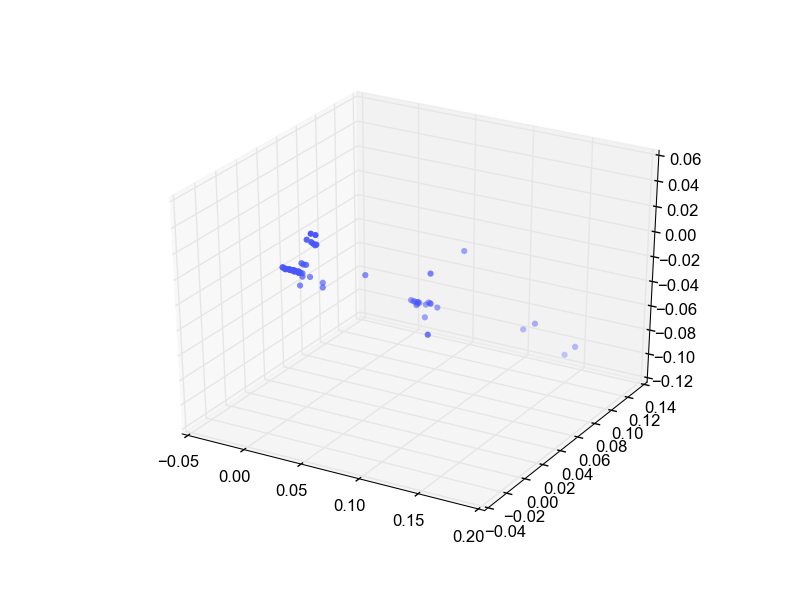
\includegraphics[width=\linewidth]{secciones/graficos/oja/categoria_1.png}
                \caption{Categoría 1}
                \label{fig: ej1_oja_categoria_1}
        \end{subfigure}
        \begin{subfigure}[b]{0.33\textwidth}
                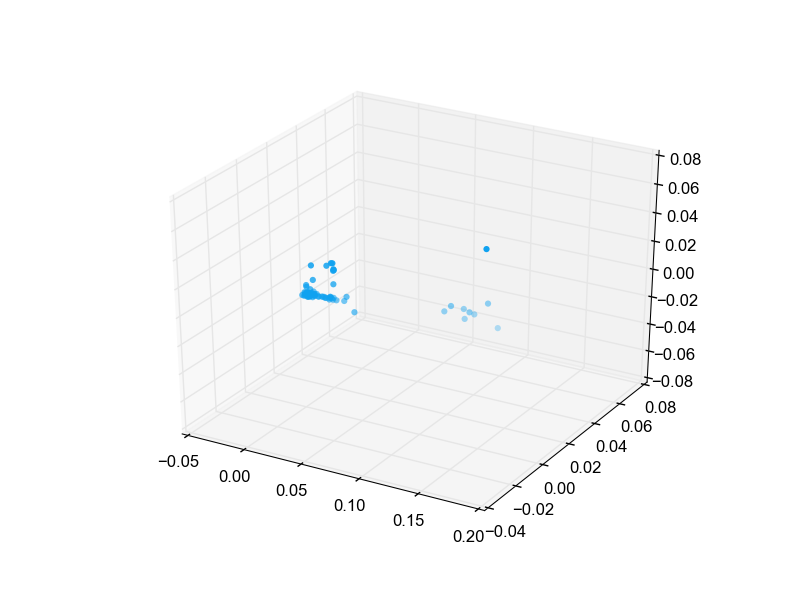
\includegraphics[width=\linewidth]{secciones/graficos/oja/categoria_2.png}
                \caption{Categoría 2}
                \label{fig: ej1_oja_categoria_2}
        \end{subfigure}
        \begin{subfigure}[b]{0.33\textwidth}
                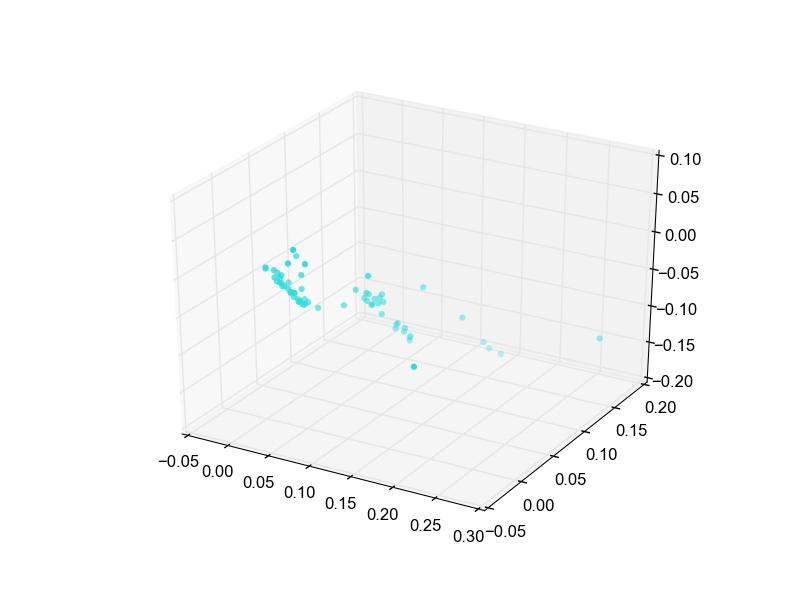
\includegraphics[width=\linewidth]{secciones/graficos/oja/categoria_3.png}
                \caption{Categoría 3}
                \label{fig: ej1_oja_categoria_4}
        \end{subfigure}
        \begin{subfigure}[b]{0.33\textwidth}
                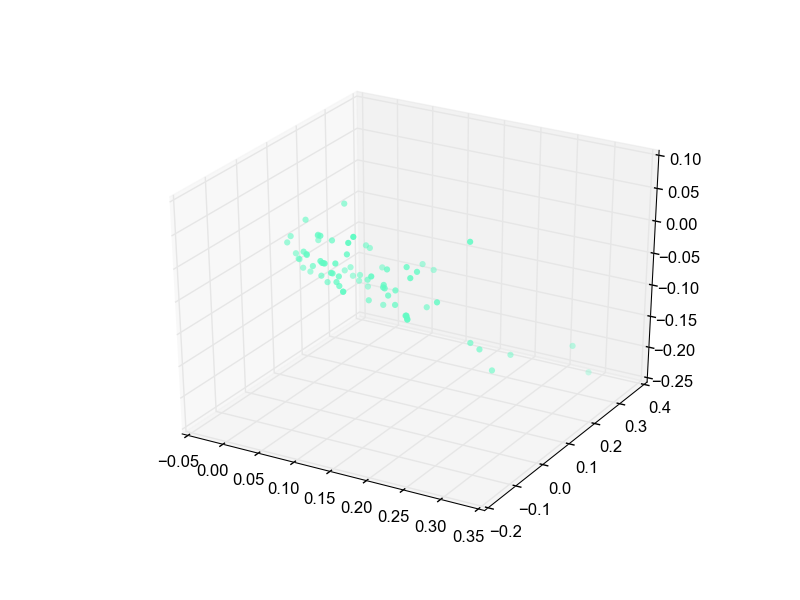
\includegraphics[width=\linewidth]{secciones/graficos/oja/categoria_4.png}
                \caption{Categoría 4}
                \label{fig: ej1_oja_categoria_4}
        \end{subfigure}
        \begin{subfigure}[b]{0.33\textwidth}
                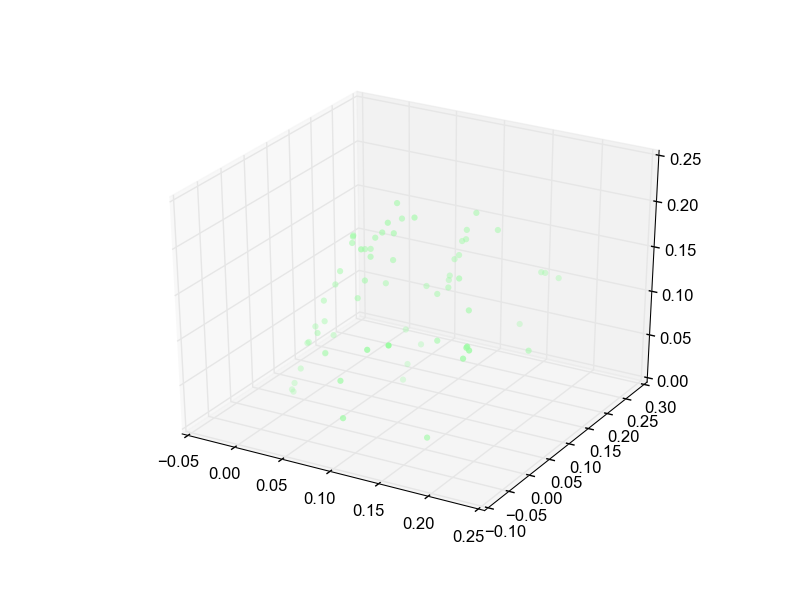
\includegraphics[width=\linewidth]{secciones/graficos/oja/categoria_5.png}
                \caption{Categoría 5}
                \label{fig: ej1_oja_categoria_5}
        \end{subfigure}
        \begin{subfigure}[b]{0.33\textwidth}
                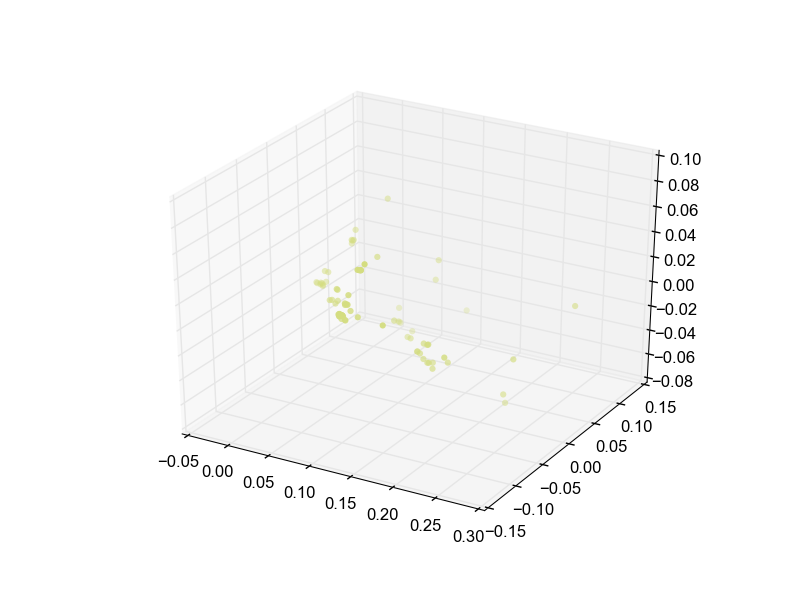
\includegraphics[width=\linewidth]{secciones/graficos/oja/categoria_6.png}
                \caption{Categoría 6}
                \label{fig: ej1_oja_categoria_6}
        \end{subfigure}
        \begin{subfigure}[b]{0.33\textwidth}
                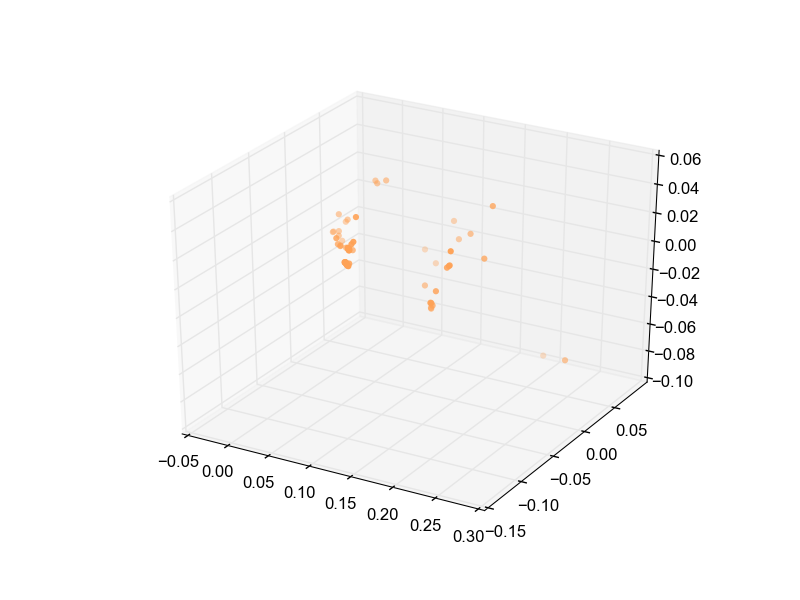
\includegraphics[width=\linewidth]{secciones/graficos/oja/categoria_7.png}
                \caption{Categoría 7}
                \label{fig: ej1_oja_categoria_7}
        \end{subfigure}
        \begin{subfigure}[b]{0.33\textwidth}
                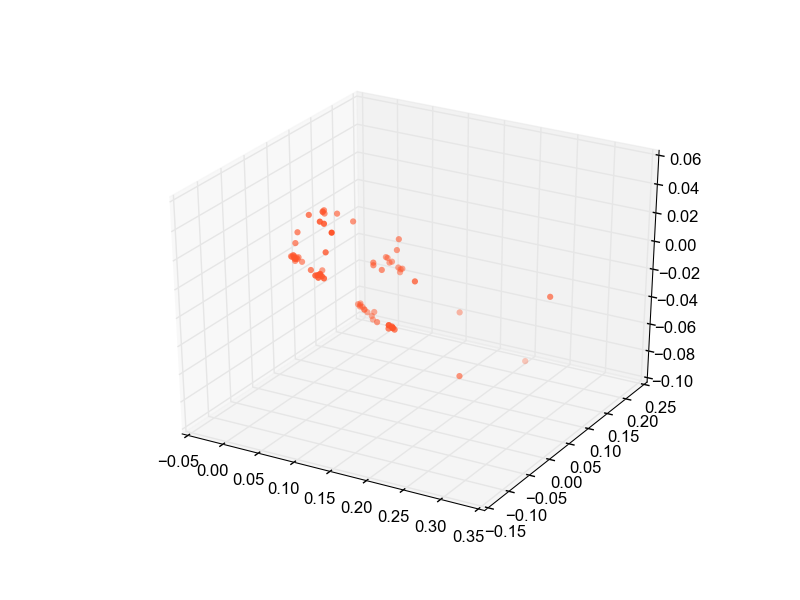
\includegraphics[width=\linewidth]{secciones/graficos/oja/categoria_8.png}
                \caption{Categoría 8}
                \label{fig: ej1_oja_categoria_8}
        \end{subfigure}
        \begin{subfigure}[b]{0.33\textwidth}
                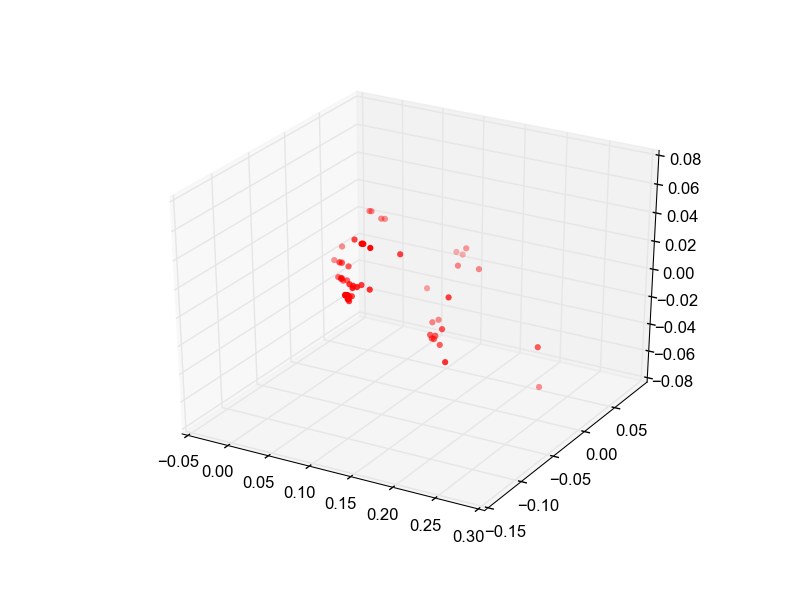
\includegraphics[width=\linewidth]{secciones/graficos/oja/categoria_9.png}
                \caption{Categoría 9}
                \label{fig: ej1_oja_categoria_9}
        \end{subfigure}
        \caption{Gráficos de resultados diferenciados por categoría}
        \label{fig: ej1_oja_categorias}
\end{figure}


\par Como observamos que algunas categorías se encontraban algo dispersas, calculamos la varianza promedio de los datos de cada categoría para ver si nos dan alguna señal de por qué puede estar ocurriendo esto. Los resultados se pueden observar en la siguiente figura \ref{fig: varianza_entrada}.

\begin{figure}[H]
        \centering
        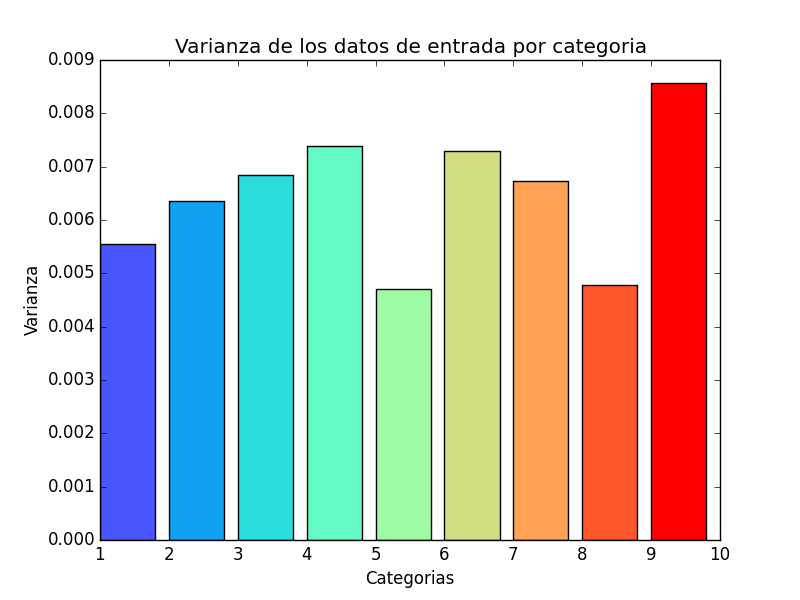
\includegraphics[width=0.8\linewidth]{secciones/graficos/varianza_entrada.png}
        \caption{Varianza de los datos de entrada por categoría}
        \label{fig: varianza_entrada}
\end{figure}

\par En la figura \ref{fig: ej1_oja_errores}, se puede observar como se satisface la condición de ortonormalidad, en función del número de época. Se aprecia que a partir de las 1000 épocas la norma se hace menor al 0.18 y continúa decreciendo fuértemente hasta valores por debajo de 0.02.


\begin{figure}[H]
        \begin{subfigure}[b]{0.5\textwidth}
                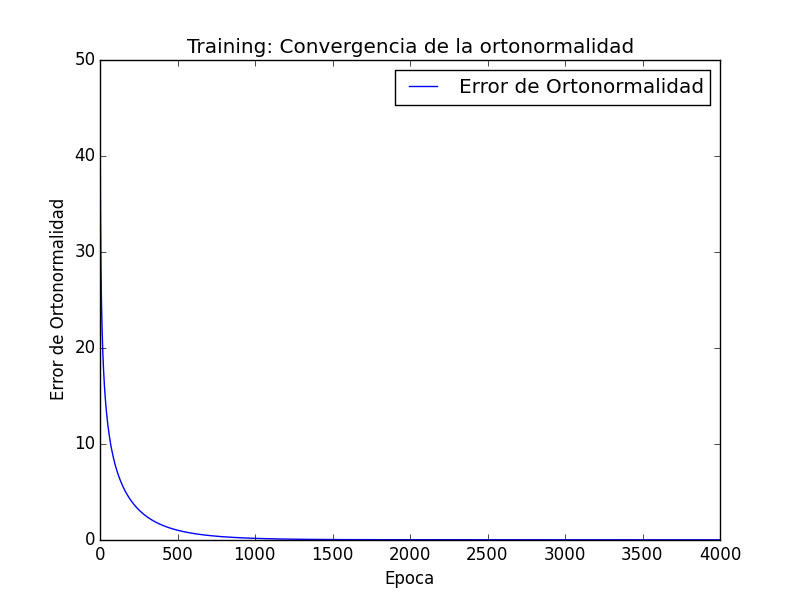
\includegraphics[width=\linewidth]{secciones/graficos/oja/error.png}
                \caption{Todas las épocas}
                \label{fig: ej1_oja_error}
        \end{subfigure}
        \begin{subfigure}[b]{0.5\textwidth}
                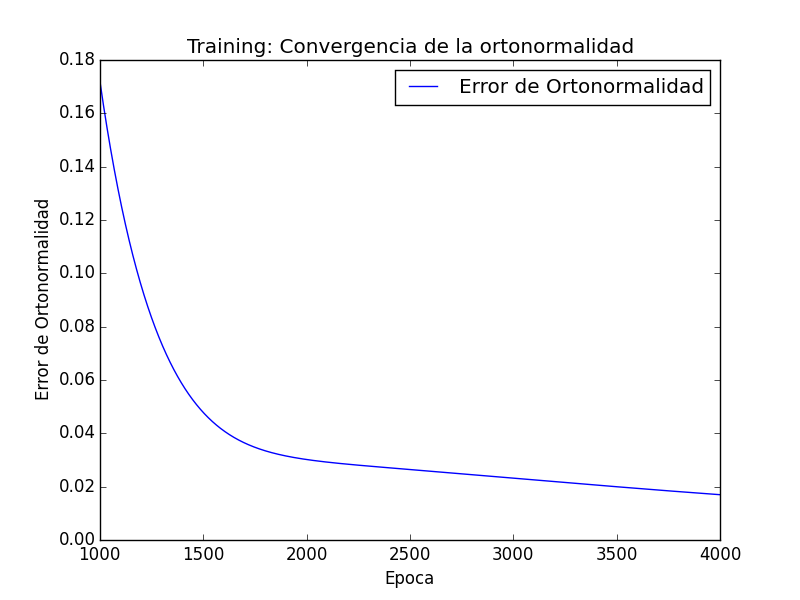
\includegraphics[width=\linewidth]{secciones/graficos/oja/error_zoom.png}
                \caption{A partir de la época 1000}
                \label{fig: ej1_oja_error_zoom}
        \end{subfigure}
        \caption{Ortonormalidad de la matriz de pesos en función de las épocas.}
        \label{fig: ej1_oja_errores}
\end{figure}


\subsubsection{Algoritmo de Sanger}

\par Se realizó una análisis similar al caso anterior, utilizando el mismo porcentaje de datos de entrenamiento - validación y el mismo coeficiente de aprendizaje adaptativo. En la figuras \ref{fig: ej1_sanger_3d_1} y \ref{fig: ej1_sanger_3d_2} se puede observar vistas 3d (componentes principales obtenidos por el algoritmo) de los datos de entrenamiento (figuras \ref{fig: ej1_sanger_3d_1_train}, \ref{fig: ej1_sanger_3d_2_train}) y validacion (figuras \ref{fig: ej1_sanger_3d_1_valid}, \ref{fig: ej1_sanger_3d_2_valid}). Al igual que en el caso anterior, obtenemos una buena clasificación sobre los datos de validación.

\begin{figure}[H]
        \begin{subfigure}[b]{0.5\textwidth}
                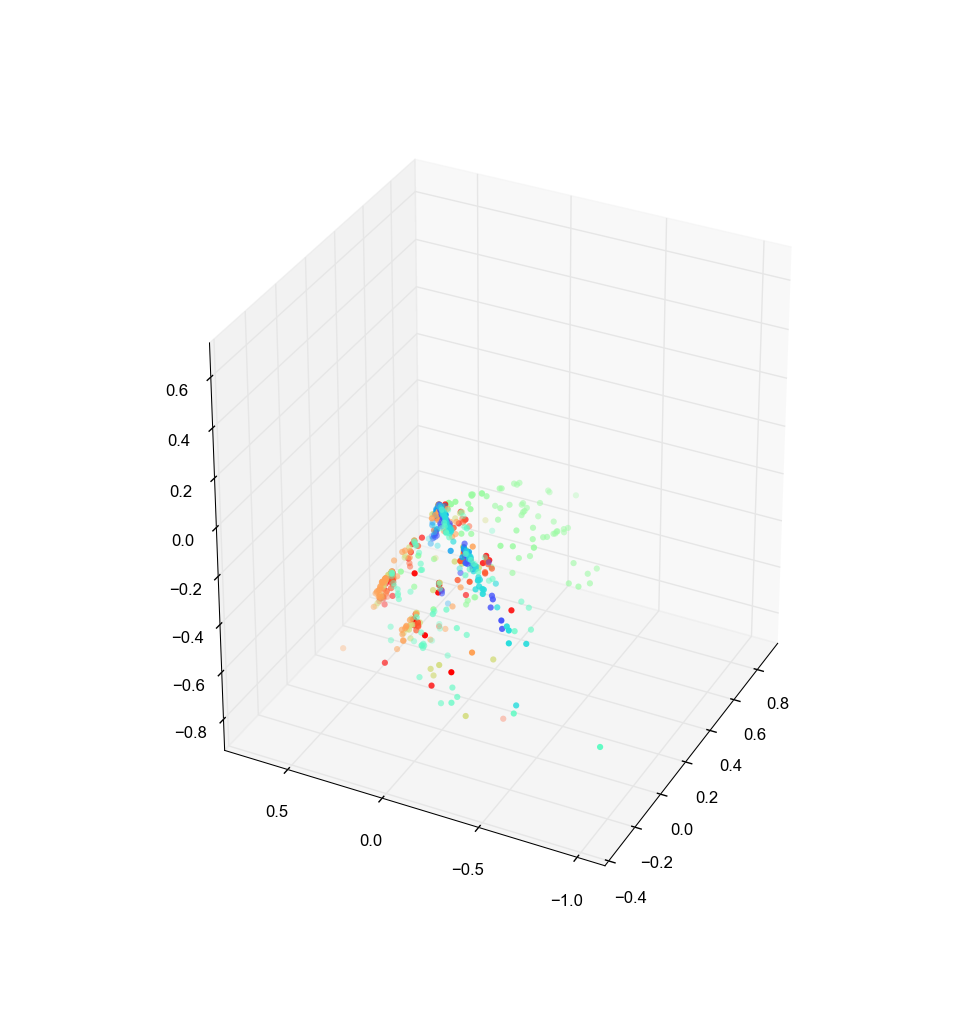
\includegraphics[width=\linewidth]{secciones/graficos/sanger/1_train.png}
                \caption{Entrenamiento}
                \label{fig: ej1_sanger_3d_1_train}
        \end{subfigure}%
        \begin{subfigure}[b]{0.5\textwidth}
                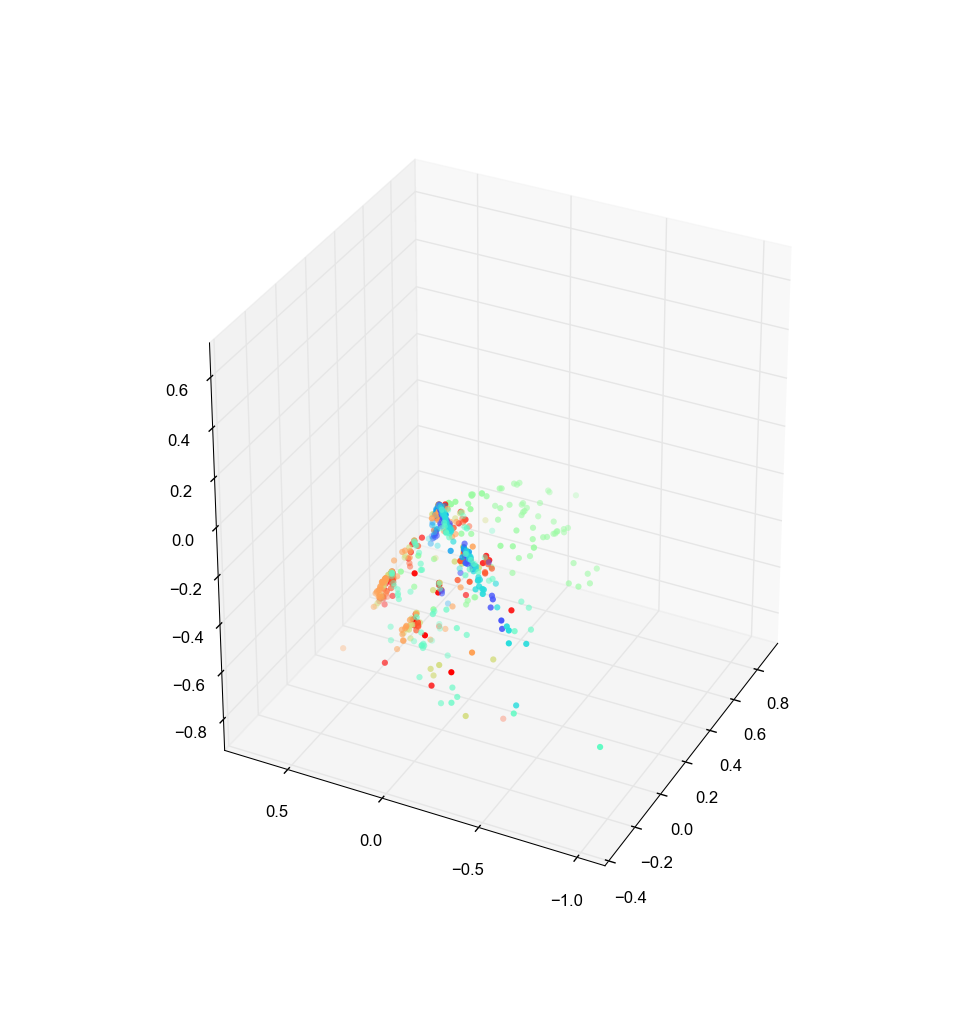
\includegraphics[width=\linewidth]{secciones/graficos/sanger/1_train.png}
                \caption{Validacion}
                \label{fig: ej1_sanger_3d_1_valid}
        \end{subfigure}
        \caption{Vista 1 en 3d de resultados de validación y entrenamiento}
        \label{fig: ej1_sanger_3d_1}
\end{figure}

\begin{figure}[H]
        \begin{subfigure}[b]{0.5\textwidth}
                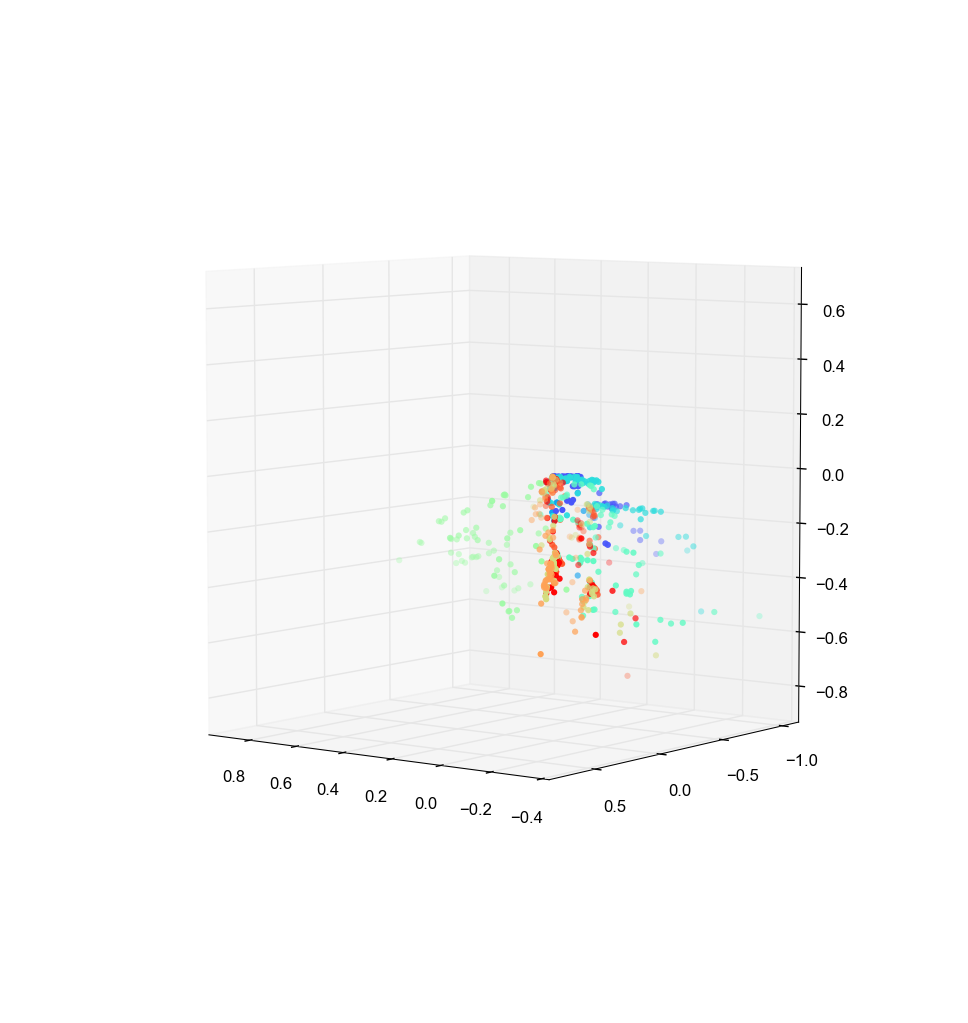
\includegraphics[width=\linewidth]{secciones/graficos/sanger/2_train.png}
                \caption{Entrenamiento}
                \label{fig: ej1_sanger_3d_2_train}
        \end{subfigure}
        \begin{subfigure}[b]{0.5\textwidth}
                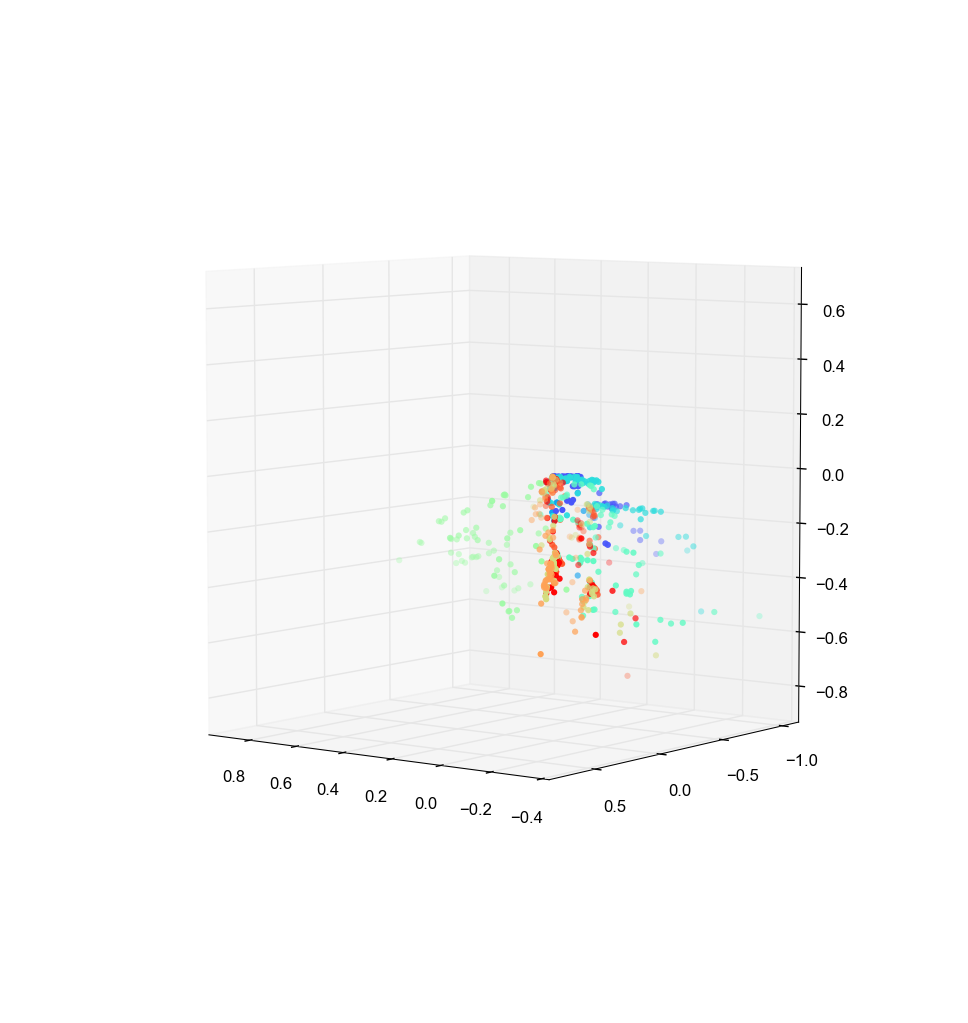
\includegraphics[width=\linewidth]{secciones/graficos/sanger/2_train.png}
                \caption{Validacion}
                \label{fig: ej1_sanger_3d_2_valid}
        \end{subfigure}
        \caption{Vista 2 en 3d de resultados de validación y entrenamiento}
        \label{fig: ej1_sanger_3d_2}
\end{figure}

\par proyectando estos gráficos 3d sobre distintos planos, obtenemos las siguientes figuras, tanto para entrenamiento figuras \ref{fig: ej1_sanger_ejes_train} como para validación figura \ref{fig: ej1_sanger_ejes_valid}

\begin{figure}[H]
        \begin{subfigure}[b]{0.33\textwidth}
                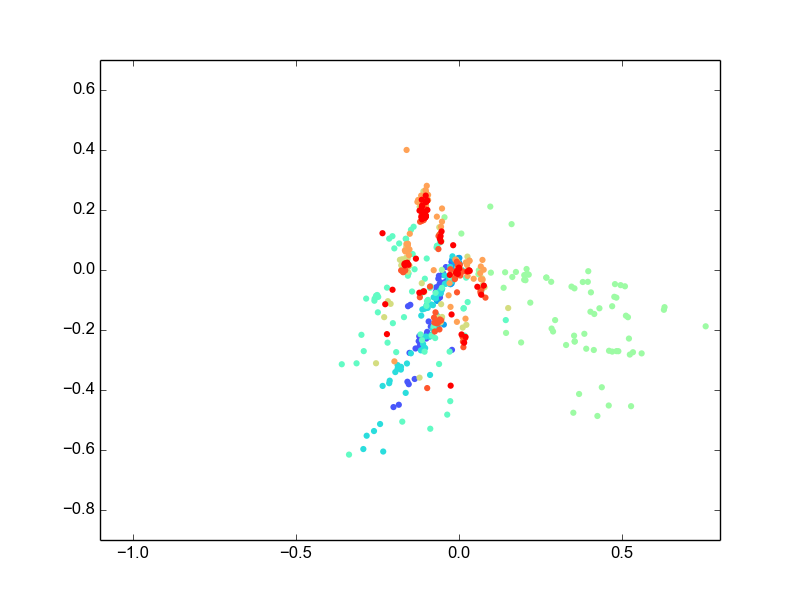
\includegraphics[width=\linewidth]{secciones/graficos/sanger/eje1_train.png}
                \caption{Corte 1}
                \label{fig: ej1_sanger_eje_1_train}
        \end{subfigure}
        \begin{subfigure}[b]{0.33\textwidth}
                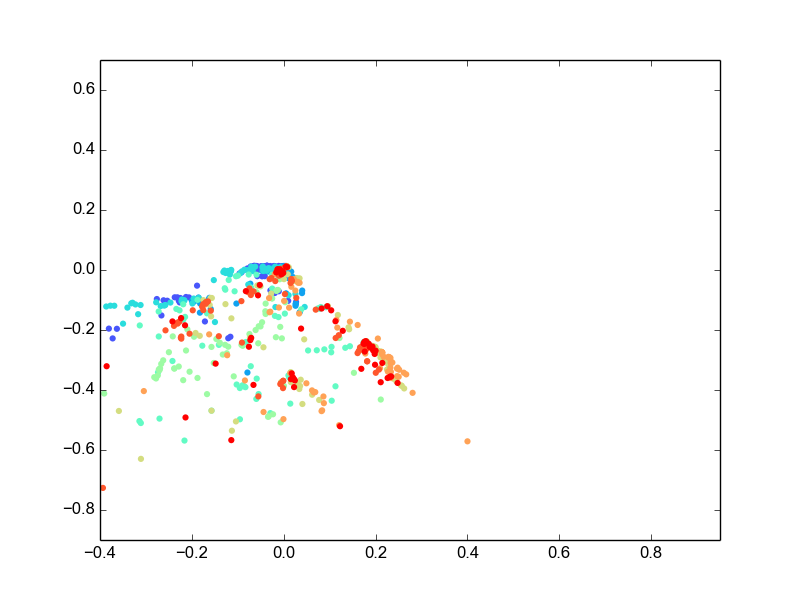
\includegraphics[width=\linewidth]{secciones/graficos/sanger/eje2_train.png}
                \caption{Corte 2}
                \label{fig: ej1_sanger_eje_2_train}
        \end{subfigure}
        \begin{subfigure}[b]{0.33\textwidth}
                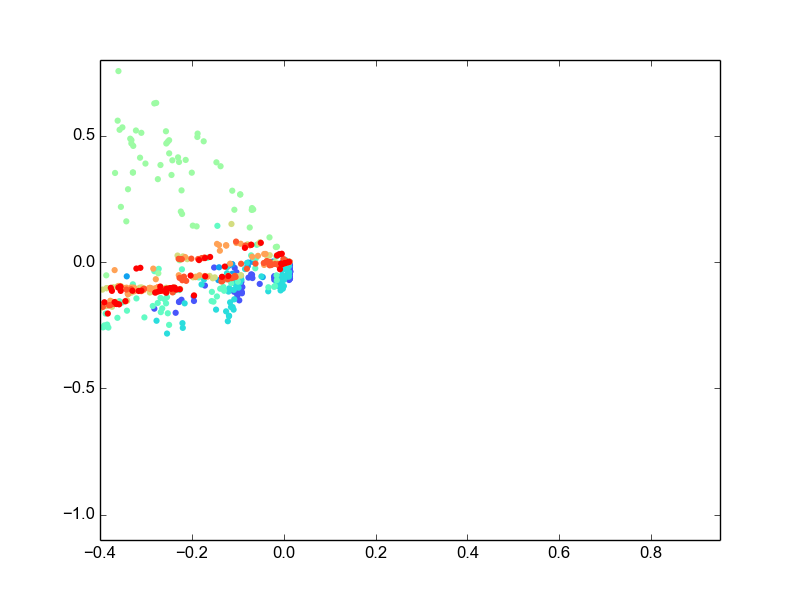
\includegraphics[width=\linewidth]{secciones/graficos/sanger/eje3_train.png}
                \caption{Corte 3}
                \label{fig: ej1_sanger_eje_3_train}
        \end{subfigure}
        \caption{Cortes del gráfico de los datos de entrenamiento}
        \label{fig: ej1_sanger_ejes_train}
\end{figure}

\begin{figure}[H]
        \begin{subfigure}[b]{0.33\textwidth}
                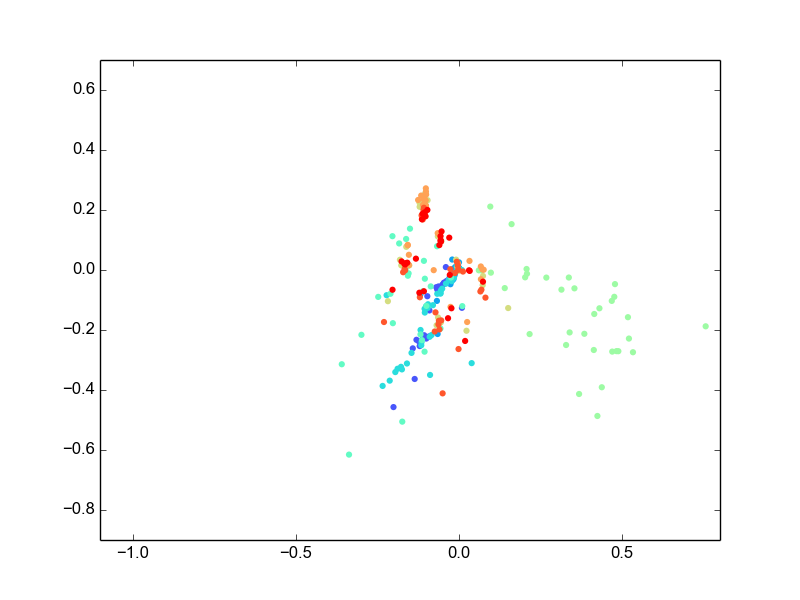
\includegraphics[width=\linewidth]{secciones/graficos/sanger/eje1_valid.png}
                \caption{Corte 1}
                \label{fig: ej1_sanger_eje_1_valid}
        \end{subfigure}
        \begin{subfigure}[b]{0.33\textwidth}
                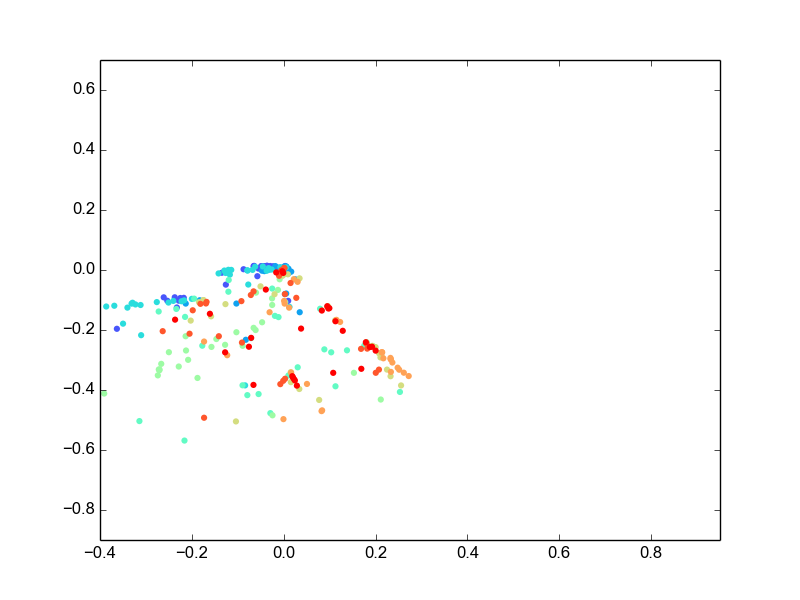
\includegraphics[width=\linewidth]{secciones/graficos/sanger/eje2_valid.png}
                \caption{Corte 2}
                \label{fig: ej1_sanger_eje_2_valid}
        \end{subfigure}
        \begin{subfigure}[b]{0.33\textwidth}
                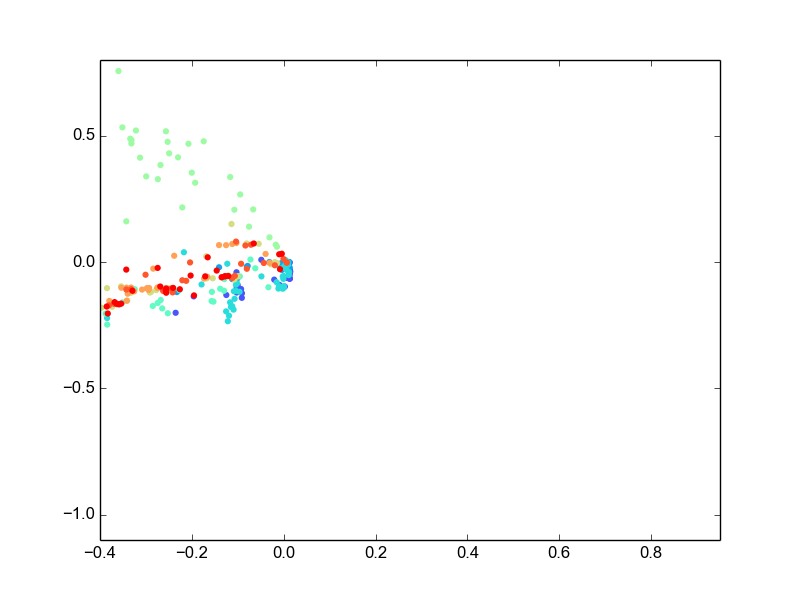
\includegraphics[width=\linewidth]{secciones/graficos/sanger/eje3_valid.png}
                \caption{Corte 3}
                \label{fig: ej1_sanger_eje_3_valid}
        \end{subfigure}
        \caption{Cortes del gráfico de los datos de validación}
        \label{fig: ej1_sanger_ejes_valid}
\end{figure}


\par A continuación podemos observar los resultados de entrenamiento en gráficos 3d para las distintas categorías, con el fin de observar más claramente como se distribuyen los mismos (figuras \ref{fig: ej1_sanger_categorias}). 

\begin{figure}[H]
        \begin{subfigure}[b]{0.33\textwidth}
                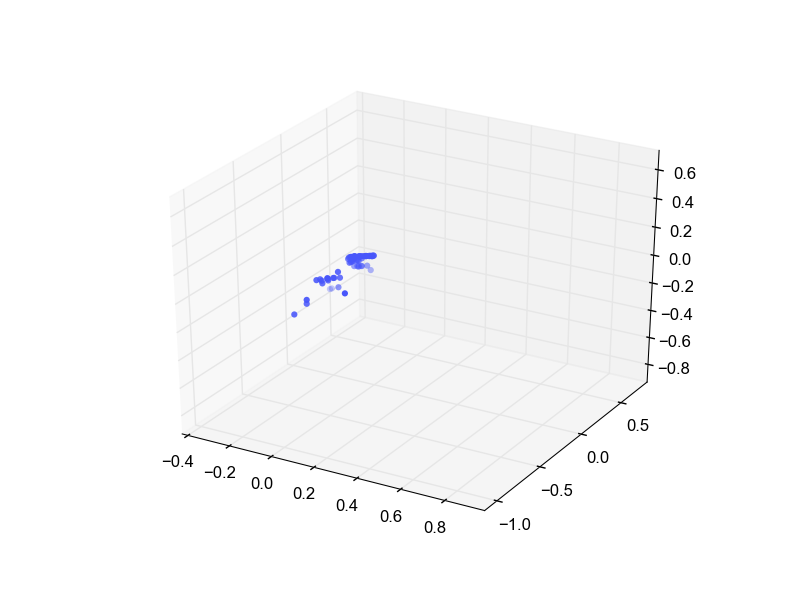
\includegraphics[width=\linewidth]{secciones/graficos/sanger/categoria_1.png}
                \caption{Categoría 1}
                \label{fig: ej1_sanger_categoria_1}
        \end{subfigure}
        \begin{subfigure}[b]{0.33\textwidth}
                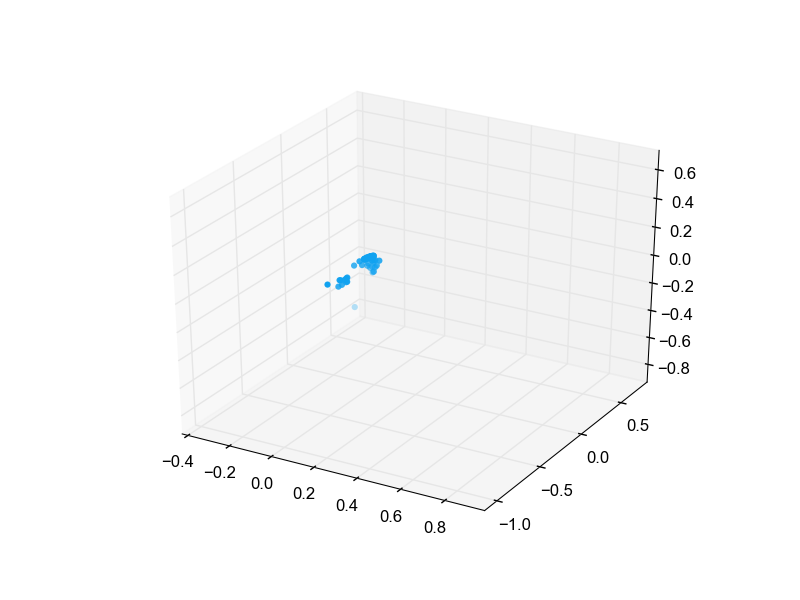
\includegraphics[width=\linewidth]{secciones/graficos/sanger/categoria_2.png}
                \caption{Categoría 2}
                \label{fig: ej1_sanger_categoria_2}
        \end{subfigure}
        \begin{subfigure}[b]{0.33\textwidth}
                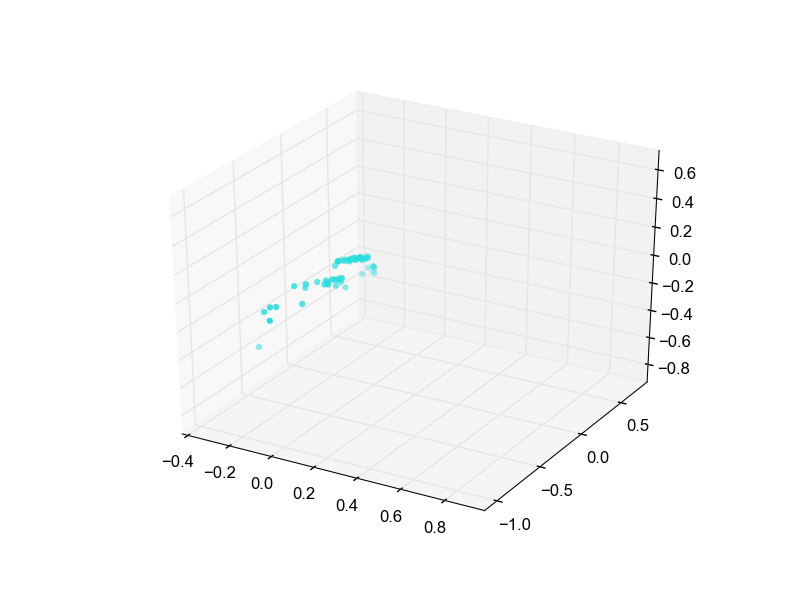
\includegraphics[width=\linewidth]{secciones/graficos/sanger/categoria_3.png}
                \caption{Categoría 3}
                \label{fig: ej1_sanger_categoria_4}
        \end{subfigure}
        \begin{subfigure}[b]{0.33\textwidth}
                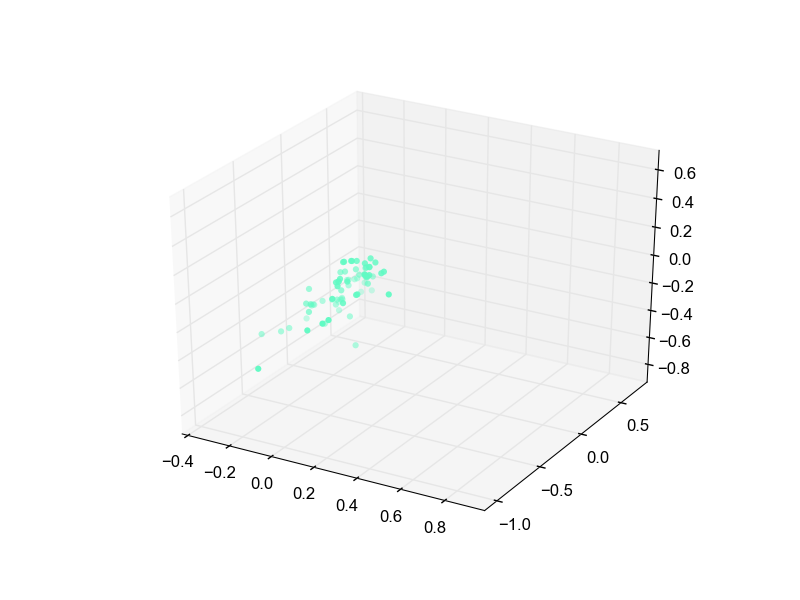
\includegraphics[width=\linewidth]{secciones/graficos/sanger/categoria_4.png}
                \caption{Categoría 4}
                \label{fig: ej1_sanger_categoria_4}
        \end{subfigure}
        \begin{subfigure}[b]{0.33\textwidth}
                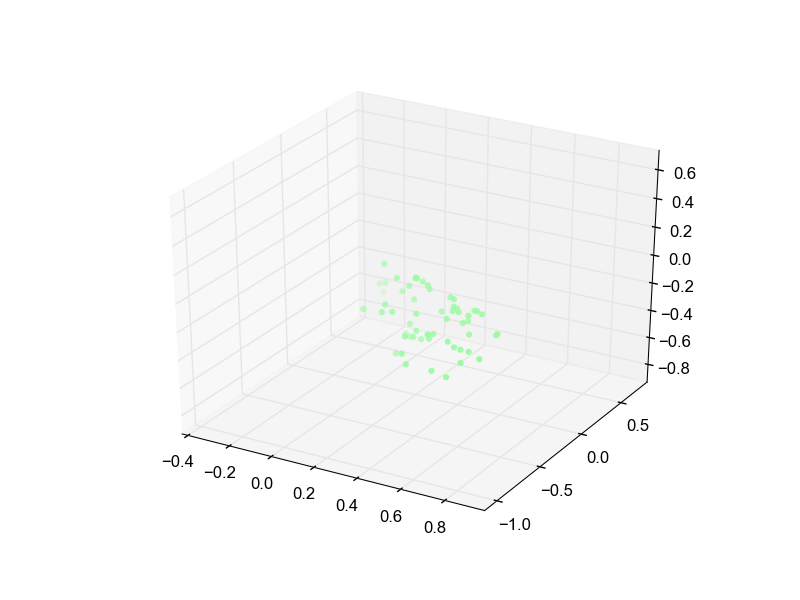
\includegraphics[width=\linewidth]{secciones/graficos/sanger/categoria_5.png}
                \caption{Categoría 5}
                \label{fig: ej1_sanger_categoria_5}
        \end{subfigure}
        \begin{subfigure}[b]{0.33\textwidth}
                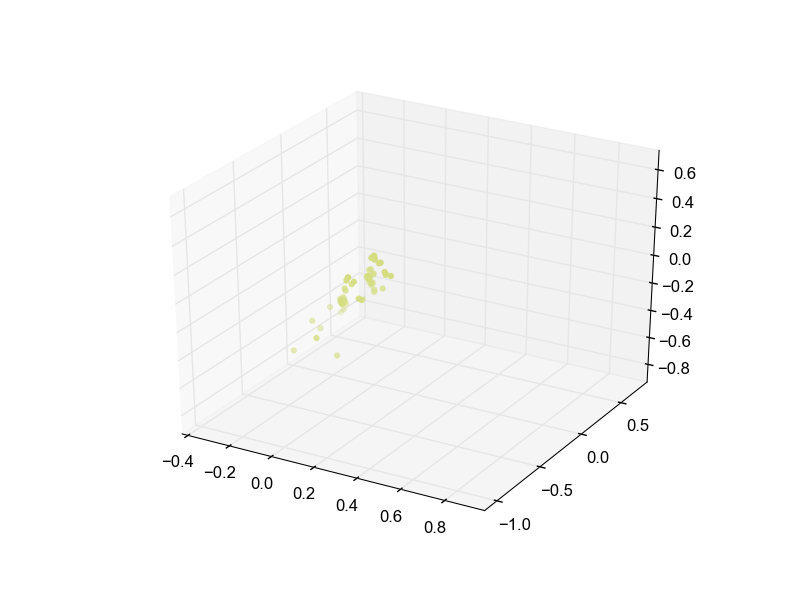
\includegraphics[width=\linewidth]{secciones/graficos/sanger/categoria_6.png}
                \caption{Categoría 6}
                \label{fig: ej1_sanger_categoria_6}
        \end{subfigure}
        \begin{subfigure}[b]{0.33\textwidth}
                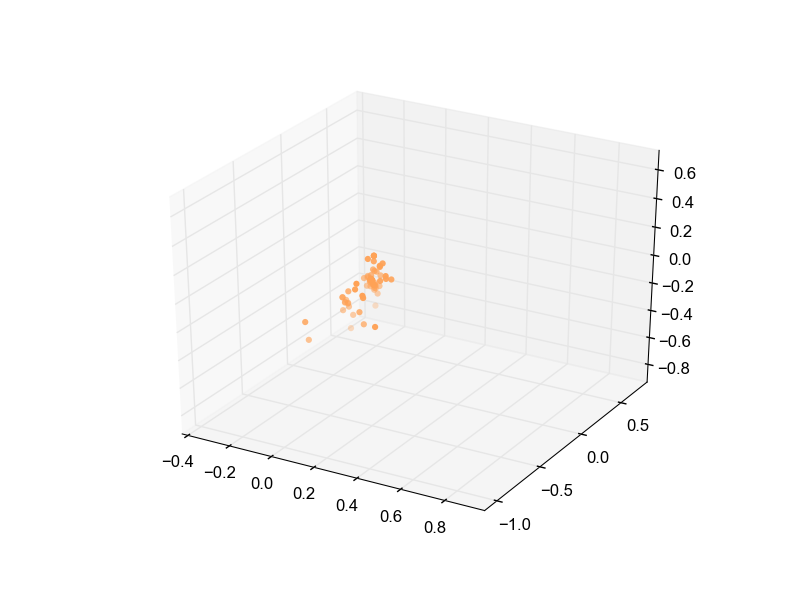
\includegraphics[width=\linewidth]{secciones/graficos/sanger/categoria_7.png}
                \caption{Categoría 7}
                \label{fig: ej1_sanger_categoria_7}
        \end{subfigure}
        \begin{subfigure}[b]{0.33\textwidth}
                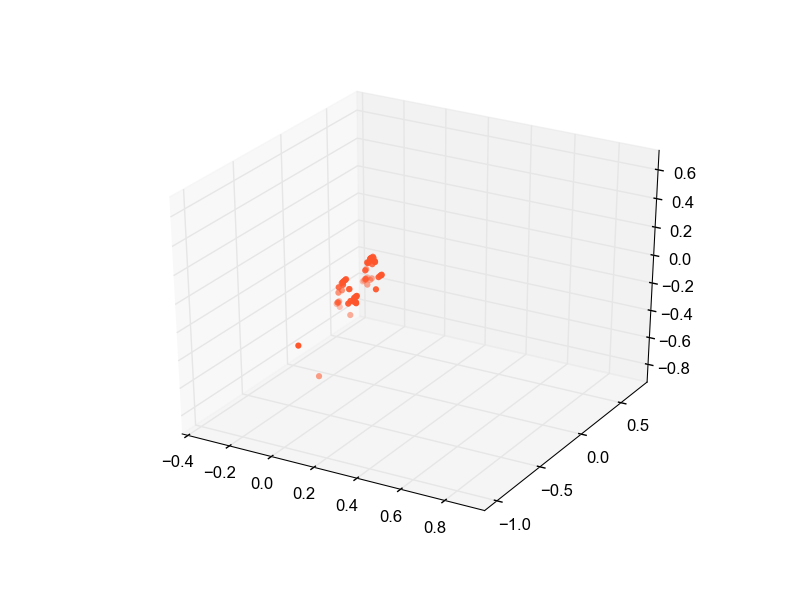
\includegraphics[width=\linewidth]{secciones/graficos/sanger/categoria_8.png}
                \caption{Categoría 8}
                \label{fig: ej1_sanger_categoria_8}
        \end{subfigure}
        \begin{subfigure}[b]{0.33\textwidth}
                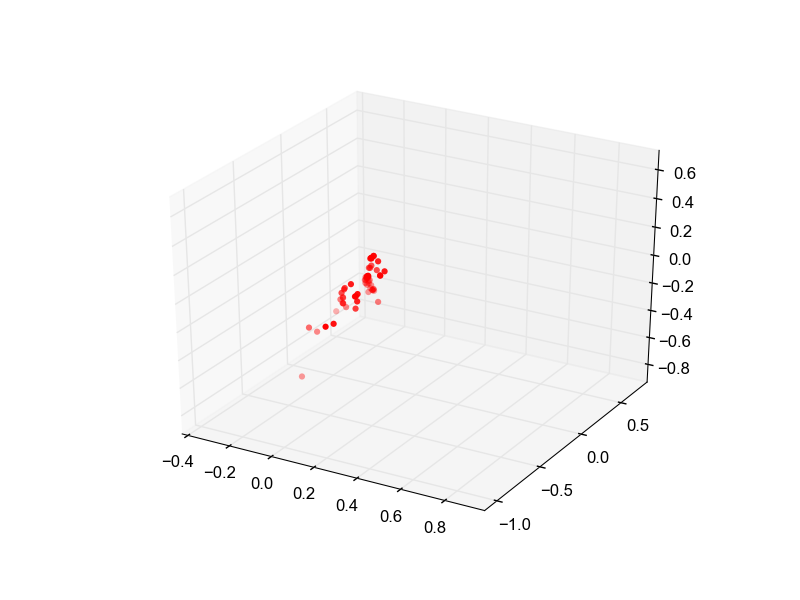
\includegraphics[width=\linewidth]{secciones/graficos/sanger/categoria_9.png}
                \caption{Categoría 9}
                \label{fig: ej1_sanger_categoria_9}
        \end{subfigure}
        \label{fig: ej1_sanger_categorias}
\end{figure}


\par Cabe destacar que los datos de entrada son los mismos tanto para Oja como para Sanger. Por lo que la varianza observada en la figura \ref{fig: varianza_entrada} también aplica para esta regla de aprendizaje y debemos tenerla en cuenta a la hora de comprender la dispersión de los datos de las categorías en los gráficos obtenidos.


\par En las figuras \ref{fig: ej1_sanger_errores}, se puede observar como se satisface la condición de ortonormalidad, en función del número de época. Se aprecia que a partir de las 1000 épocas la norma se hace menor al 0.0004, un valor muy bajo, y continúa decreciendo.

\begin{figure}[H]
        \begin{subfigure}[b]{0.5\textwidth}
                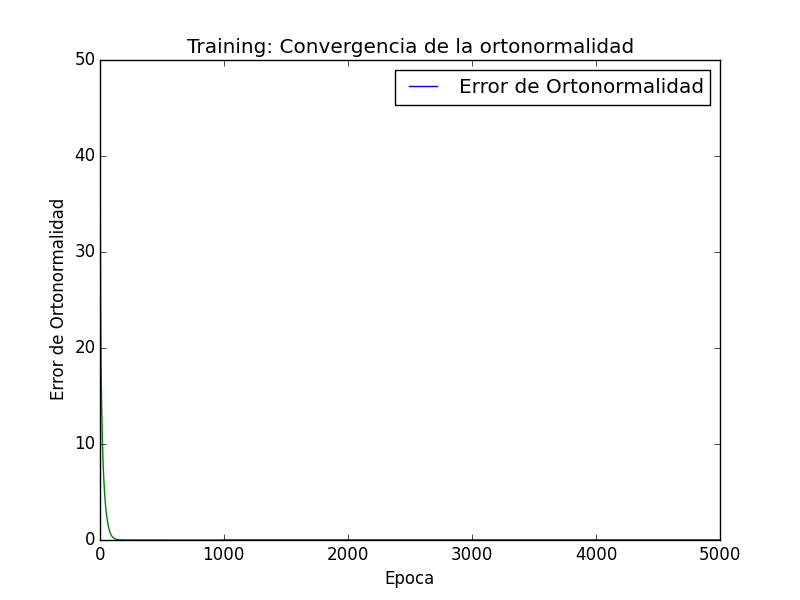
\includegraphics[width=\linewidth]{secciones/graficos/sanger/error.png}
                \caption{Todas las épocas}
                \label{fig: ej1_sanger_error}
        \end{subfigure}
        \begin{subfigure}[b]{0.5\textwidth}
                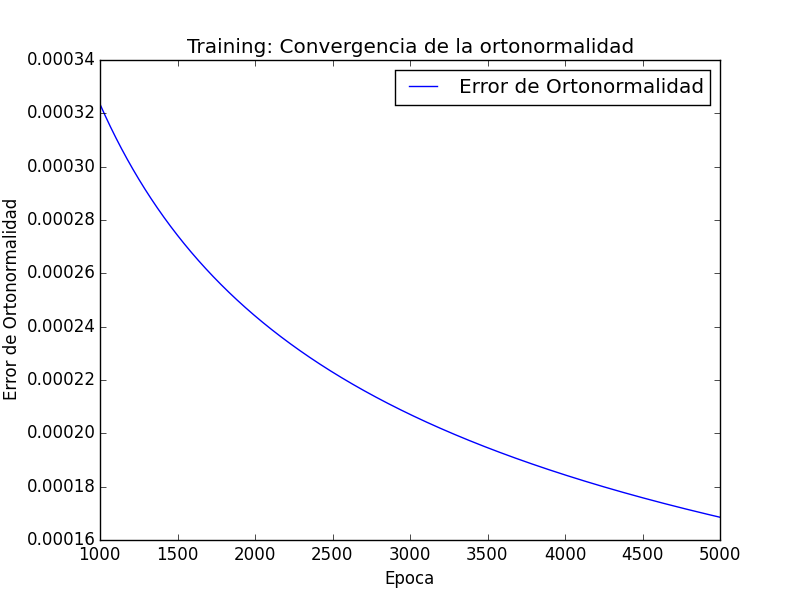
\includegraphics[width=\linewidth]{secciones/graficos/sanger/error_zoom.png}
                \caption{A partir de la época 1000}
                \label{fig: ej1_sanger_error_zoom}
        \end{subfigure}
        \caption{Ortonormalidad de la matriz de pesos en función de las épocas.}
        \label{fig: ej1_sanger_errores}
\end{figure}

\subsection{Conclusiones}

\par Se implementaron dos algoritmos para reducir la dimensionalidad del set de datos de entrada. Tanto el algoritmo de Sanger como el de Oja nos permiten obtener una clasificación que es consistente con los datos de validación. La diferencia entre los algortimos radica en que el de sanger nos permite obtener las componente principales, mientras que el de oja nos da un subespacio generado por estos, pero no nos da explicitamente las direcciones. Contrario a lo esperado, no pudimos visualizar esta diferencia. 



\section{Mapeo de Características}

Esta etapa del trabajo consiste en la implementación de un \textbf{mapa
de características} para la clasificación de las palabras según
la \textbf{categoría} que les fue asignada previamente.

Lo que se espera obtener es un \textbf{mapa auto-organizado} en el cual
cada \textbf{categoría} este claramente diferenciada.

Para lograr el objetivo presentaremos un \textbf{mapa auto-organizado} 
basado en el algoritmo de \emph{Kohonen}.

Detalleremos los pasos que realizamos para la implementación de la solución,
la elección de la implementación y las dificultades que nos topamos al
implementarlo.

Dividimos el informe en las siguientes secciones:

\begin{itemize}
\item Implementación del Algoritmo: detallamos de forma introductoria la
implementación del algoritmo. En las siguientes etapas discutiremos los pasos
hacia la implementación final.
\item Dimensiones Adecuadas: discutimos las alternativas para la dimensión
del mapa.
\item Vecindad, Learning Rate y Sigma: discutimos las alternativas que
estudiamos para seleccionar los parámetros.
\end{itemize}

\subsection{Implementación del Algoritmo}

Para implementar la solución tomamos el algoritmo de mapas
de \emph{Kohonen} visto en clase.

La versión que implementamos es la que realiza los calculos 
por \textbf{columna}, esta versión demora mas en los calculos 
que la versión matricial, pero su implementación nos resulto mas 
sencilla.

Tomamos una dimensíón del mapa de 20 x 20 y para la actualización 
de las vecindades utilizamos la \textbf{función gaussiana} con un 
\textbf{learning rate adaptativo}. Comenzando con un radio de 
vecindad de 10.

Para el entrenamiento utilizamos dos tipos de cota, una por \textbf{cantidad
de epocas} y la otra por \textbf{la diferencia de la norma de la matriz de pesos
entre dos epocas distintas}, cuando es menor a un delta se finaliza 
el entrenamiento.


\subsection{Preprocesamiento de Datos}

Analizando el \textbf{dataset} notamos que los datos son muy esparsos, hay gran cantidad
de valores en 0 y muy pocos datos númericos.

Como primer medida corrimos el algoritmo con los datos sin procesar, luego
los estandarizamos tomando varianza: 0 y sigma: 1. Pero no hubo mejoras en la
clasificación.

El siguiente intento fue dividir los datos por 10, para llevarlo a valores entre
0 y 1, pero luego descartamos esta opción ya que no soportaría leves cambios 
en las escalas del \textbf{dataset}, al agregar algun parámetro de mayor magnitud.

Entonces decidimos dejar el \textbf{dataset} sin procesar y trabajar con los datos como
vienen.


\subsection{Dimensiones Adecuadas}

Buscamos una dimensión adecuada para el mapa, conociendo que queremos
clasificar 900 datos en 9 categorías.

Probamos con las siguientes dimensiones:

\begin{itemize}
	\item 10 x 10
	\item 20 x 20
	\item 30 x 30
\end{itemize}

\subsubsection{Dimensión 10 x 10 }

Obtuvimos que el mapa no era lo suficientemente grande y los valores de
entrada se solapaban mucho, como lo muestra la figura:

\begin{figure}[H]
  \centering
  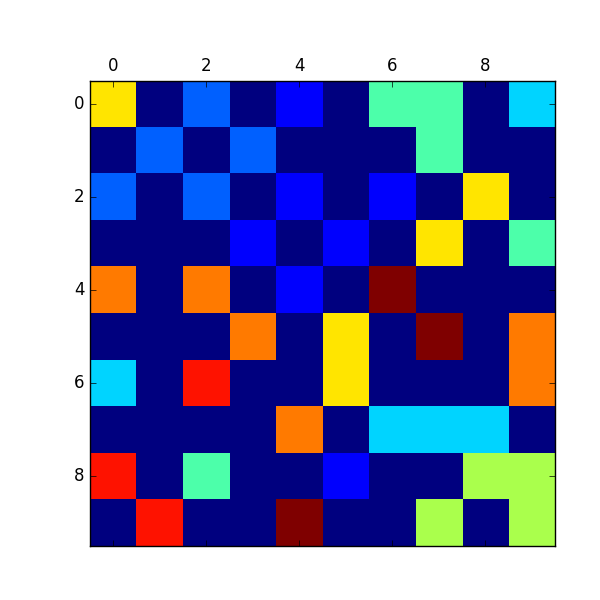
\includegraphics[width=0.5\columnwidth]{secciones/graficos/kohonen/mapa1010.png}
  \caption{Mapa 10 x 10 para 200 entradas.}
  \label{fig:mapa 10 10 200}
\end{figure}


Por lo tanto descartamos esta configuración

\subsubsection{Dimensión 20 x 20 }

Con estas dimensiones obtuvimos una buena distribución de las categorías,
aunque hay un porcentaje de neuronas que no se activaron.

\begin{figure}[H]
  \centering
  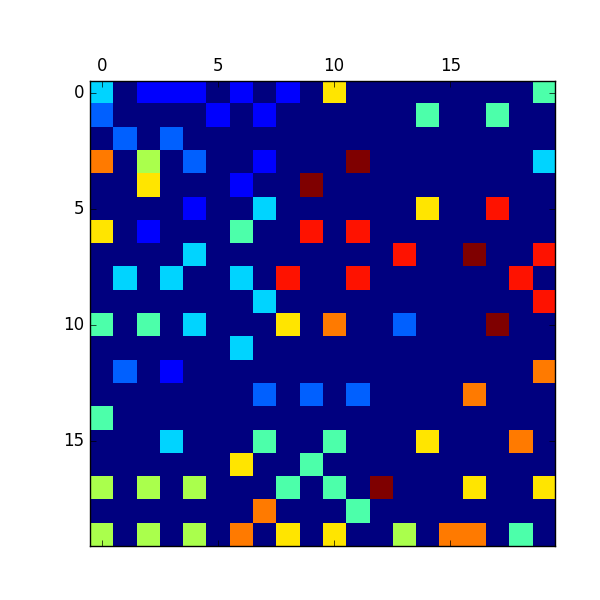
\includegraphics[width=0.5\columnwidth]{secciones/graficos/kohonen/mapa2020.png}
  \caption{Mapa 20 x 20 para 200 entradas.}
  \label{fig:mapa 20 20 200}
\end{figure}


\subsubsection{Dimensión 30 x 30 }

Para esta configuración obtuvimos mayor desperdicio de neuronas,
es decir el porcentaje que nunca se activo fue muy alto, como lo muestra
la siguiente figura

\begin{figure}[H]
  \centering
  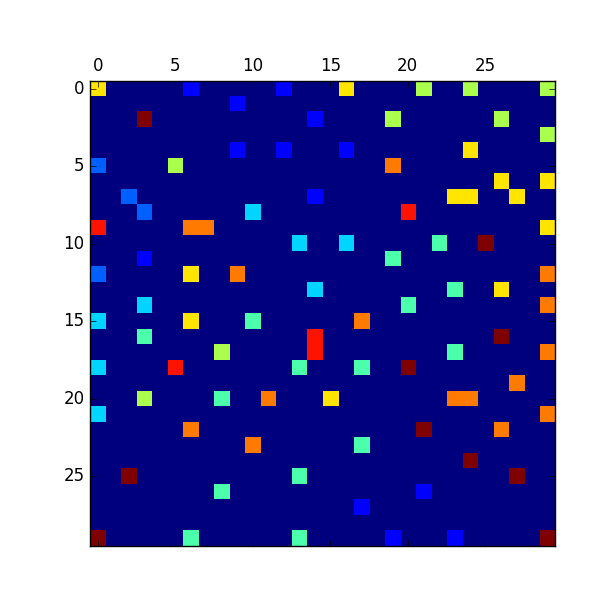
\includegraphics[width=0.5\columnwidth]{secciones/graficos/kohonen/mapa3030.png}
  \caption{Mapa 30 x 30 para 200 entradas.}
  \label{fig:mapa 30 30 200}
\end{figure}


\subsubsection{Conclusión sobre la Dimensiones}


La que mejor se adapta a las características del problema, es la
de dimensión de 20 x 20.


\subsection{Vecindad, Learning Rate y Sigma}

Para la elección de estos parametros consideramos las siguientes
alternativas:

\textbf{Vecindad} por:

\begin{itemize}
	\item Escalones: influenciamos vecinos a distancia n formando
un cuadrado.
	\item Función Gaussiana: influenciamos n vecinos utilizando
una función gaussiana.
\end{itemize}


\textbf{Learning Rate} por:

\begin{itemize}
	\item Basado en la cantidad de epocas: definimos el learning
rate basado en la cantidad de epocas aplicadas a una función.
	\item Coeficientes adaptativos: definimos un valor de
learning rate inicial y lo disminuimos a traves de coeficientes.
	\item Decrecimiento porcentual: Definimos un valor de 
learning rate inicial y por epoca lo decrementamos en un 0.X por ciento.
\end{itemize}

Para el \emph{Learning Rate} basados en la \textbf{Cantidad de Epocas}, probamos con 
las siguientes funciones: $\frac{1}{t^\frac{-1}{2}}$ y $\frac{1}{t^\frac{-1}{3}}$.


En el caso de \textbf{Coeficientes Adaptativos}, probamos con:
learning rate inicial / (1 + epoca actual * coeficiente * learning rate inicial)

Y para del \textbf{Decrecimiento Porcentual}: por cada epoca learning rate inicial * 0.X


\textbf{Sigma} por:

Definimos un valor de $sigma inicial$, lo suficientemente grande para influenciar a todo 
el mapa. Y variandolo con las epocas con dos alternativas:

\begin{itemize}
	\item $sigmaInicial * {epocaActual^\frac{-1}{3}}$
	\item $sigmaInicial * e^\frac{epocaActual}{lambd}$
\end{itemize}

Tomando como lambd: $cantidadEpocas * cantidadDatosEntrenamiento / log (sigmaInicial)$


\subsubsection{Buscando la Combinación Ideal}

Realizamos una bateria de prueba tomando un set de datos de 300 valores, para
estudiar cual de la siguiente combinación de parametros organizaba mejor
las categorías.

Primero definimos un sigma inicial: (dimensión mapa)$ / 2$, así en las primeras
epocas gran parte del mapa seria influenciado.

De las primeras pruebas concluimos que el \emph{Learning Rate} basado en la 
\textbf{cantidad de epocas} resultaba no ser una buena elección, ya que
decrece de forma muy rápido sin dar el tiempo suficiente para aprender.
Entonces descartamos esta opción.

Entonces utilizamos las otras dos opciones, definiendo un \emph{Learning Rate}
alto con valor de 0.999. En el caso de \textbf{Decrecimiento Porcentual}
tuvimos el inconveniente de que o decrecía muy rápido o demasiado lento, haciendo
dificil encontrar el punto justo.

El que nos permitió encontrar el balance fue \textbf{Coeficientes Adaptativos}
tomando como coeficiente = 0.5.

La función de \textbf{Sigma} basada en $sigmaInicial * e^\frac{epocaActual}{lambd}$
nos dió que decrecia de forma muy rápido, impidiendo el aprendizaje.
La función $sigmaInicial * {epocaActual^\frac{-1}{3}} combinado al \emph{Learning Rate}$
de tipo \textbf{adaptativo} nos dió un buen balance.

Para la función de vecindad decidimos quedarnos con la \textbf{función uniforme} ya
que presentaba una distribución más ármonica.

\subsubsection{Conclusiones de los Parámetros}

La combinación que nos resulto mejor fue tomar:


\begin{itemize}
	\item Sigma Inicial = 10
	\item Learning Rate Adaptativo =$ 0.999 / (1 + epoca_actual * 0.5 * 0.999)$
	\item Sigma = Sigma Inicial *$ {epocaActual^\frac{-1}{3}}$
\end{itemize}


\subsection{Cotas}

Para finalizar el entrenamiento definimos dos tipos de cotas:

\begin{itemize}
	\item Epocas
	\item Norma
\end{itemize}

La basada en la cantidad de \textbf{Epocas} establece una cantidad máxima de
ciclos de entrenamiento.

La basada en la \textbf{Norma} calcula la norma de la matriz de pesos (W) 
correspondiete a la epoca actual, hace la diferencia con la epoca anterior.
En caso que sea menor a una epsilon termina el entrenamiento. La ventaja
de esta es que cuando los pesos se modifican de forma despreciable entre
dos epocas significa que el aprendizaje comienza a estancarse.


\subsection{Entrenamiento}

Con los parametros seleccionados procedemos a realizar el entrenamiento de
nuestro mapa, para esto nos queda determinar la cantidad de datos con los que
conviene entrenar y estudiar si hay alguna diferencia variando las entradas
y las cotas con las que se finaliza el entrenamiento.

Tomamos distintos valores de entrada para entrenar, realizamos los test, y
reentrenamos el mapa nuevamente durante 3 etapas.

Con estas pruebas esperamos ver con que cantidad de datos de entrenamiento, 
con cual de las cotas y si la repetición influyen en la calidad de los resultados.

Al ingresar el parametro de entrenamiento, se toma una porción del dataset correspondiente
a la cantidad de entradas de forma random.

Los resultados del entrenamiento, los clasificamos en 3 categorías \textbf{Bien}, \textbf{Mal}
y \textbf{Sin Determinar} esta última corresponde a que existen dos o mas categorias a la que
podría pertenecer.



\subsubsection{50 Datos de Entrada}

Primero realizamos una prueba para ver si tomando un pequeña cantidad de datos alcanza para
categorizar todos los valores de una forma eficiente.

Configuramos los siguientes parametros como cotas:

\begin{itemize}
	\item Cantidad Máxima de Epocas = 1000
	\item Cota de la norma = 0.00001
	\item Learning Rate = 0.999
\end{itemize}


Y ejecutamos la función de entrenamiento.

Al finalizar consumió las 1000 epocas, y manteniendo una diferencia den la norma del orden 0.008 
y disminuyendo, eso quiere decir que si bien gran parte se había agrupado, todavía podía seguir
corrigiendose.

Guardamos el mapa de entrenamiento y repetimos el proceso para el mismo mapa dos veces mas,
para analizar si el entrenamiento en etapas produce mejoras.

En las dos etapas siguientes nuevamente volvio a consumir las 1000 epocas de entrenamiento,
sin alcanzar la cota de la norma.

En cada etapa ejecutamos la función \textbf{Test} y volcamos los resultados obtenidos 
de la clasificación en una tabla:


\begin{table}[htbp]
	\begin{center}
	\begin{tabular}{|l|l|}
		\hline
		Etapa & Bien & Mal & Sin Determinar 	\\
							\hline \hline
		1     & 494  & 388 & 18 		\\ \hline
		2     & 526  & 299 & 75 		\\ \hline
		3     & 522  & 344 & 34			\\ \hline
	\end{tabular}
	\caption{Resultados de Validación}
	\label{tabla:entrenamiento 50 entradas}
	\end{center}
\end{table}

Como se puede ver en entrenamiento mejoró levemente respecto a la primer etapa, para la 
tercera se generó una disminución respecto a los aciertos, pero una mejor clasificación
de los incorrectos.

Presentamos el mapa obtenido del entramiento para la tercera etapa.


\begin{figure}[H]
  \centering
  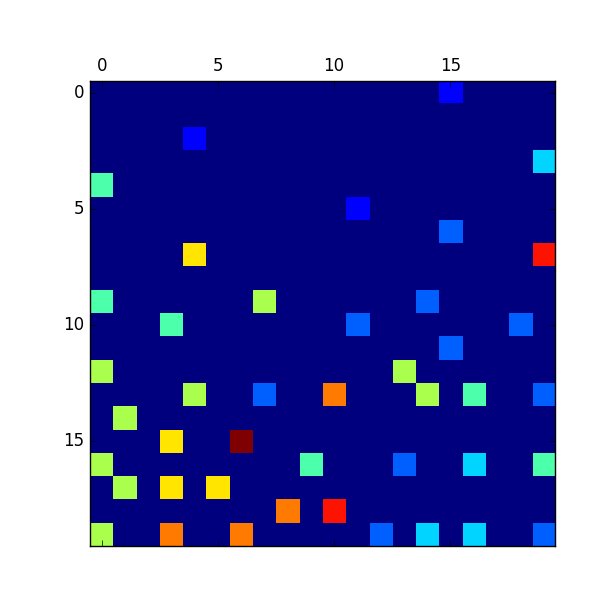
\includegraphics[width=0.5\columnwidth]{secciones/graficos/kohonen/mapaentrenamiento50.png}
  \caption{Mapa de Entrenamiento para 50 entradas.}
  \label{fig:mapa train 50}
\end{figure}



Para detectar las áreas que fueron mejor clasificadas, graficamos el mapa de
los aciertos.

\begin{figure}[H]
  \centering
  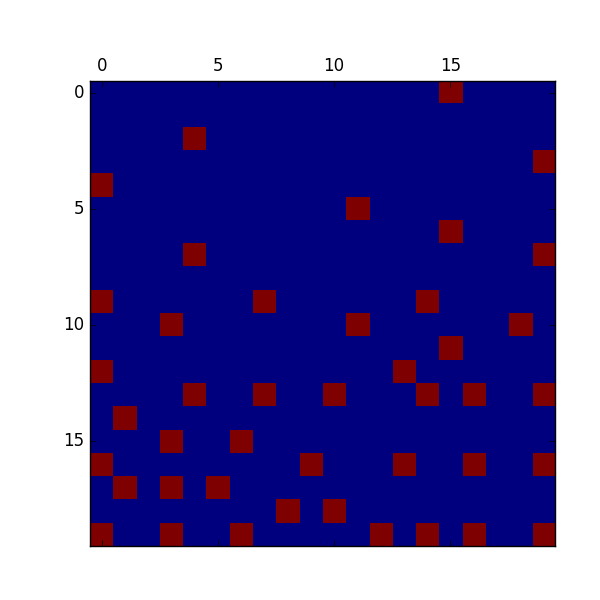
\includegraphics[width=0.5\columnwidth]{secciones/graficos/kohonen/mapaaciertos50.png}
  \caption{Mapa de Aciertos para 50 entradas.}
  \label{fig:mapa aciertos 50}
\end{figure}

Hacemos lo mismo con los datos mal clasificados.

\begin{figure}[H]
  \centering
  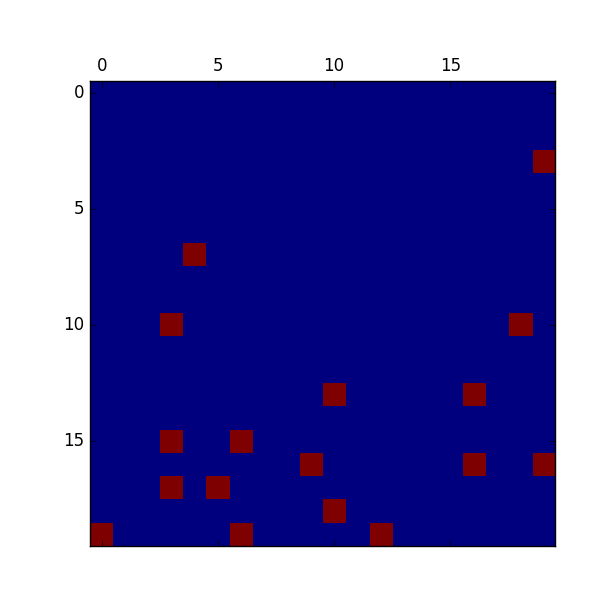
\includegraphics[width=0.5\columnwidth]{secciones/graficos/kohonen/mapaerrores50.png}
  \caption{Mapa de Errores para 50 entradas.}
  \label{fig:mapa errores 50}
\end{figure}


Y para los datos sin determinar.

\begin{figure}[H]
  \centering
  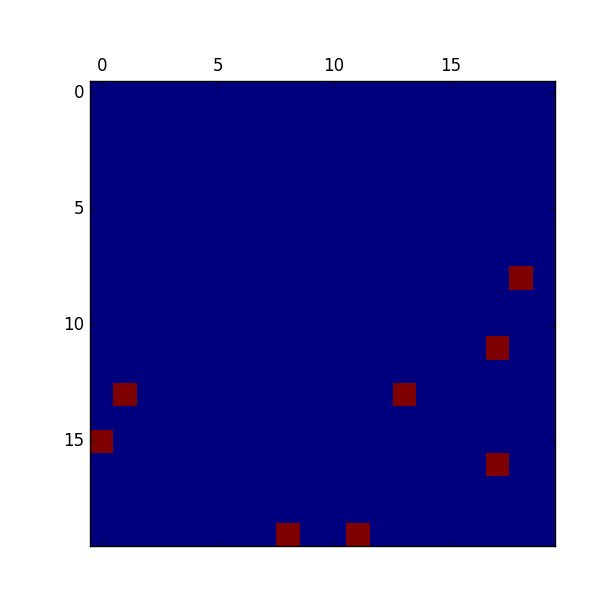
\includegraphics[width=0.5\columnwidth]{secciones/graficos/kohonen/mapaindefinidas50.png}
  \caption{Mapa de Indefinidos para 50 entradas.}
  \label{fig:mapa indefinidos 50}
\end{figure}


Como se puede ver la mayor cantidad de malas clasificaciones y e imposibilidad
de clasificar se da en el área donde las neuronas no llegaron a organizarse completamente.


\subsubsection{200 Datos de Entrada}

Incrementamos los datos de entrenamiento, con la premisa de que un mayor set de entrenamiento
va a mejorar la clasificación.

Asique configuramos el algoritmo con los siguientes parametros para 200 datos


\begin{itemize}
	\item Cantidad Máxima de Epocas = 300
	\item Cota de la norma = 0.00001
	\item Learning Rate = 0.999
\end{itemize}

Disminuimos la cantidad de épocas, ya que al ser mas datos, pensamos que se organizarían mas 
rápido.

Corrimos el entrenamiento y nos consumió las 300 épocas. Guardamos el mapa y repetimos para 
una siguiente etapa con la configuración

\begin{itemize}
	\item Cantidad Máxima de Epocas = 500
	\item Cota de la norma = 0.00001
	\item Learning Rate = 0.999
\end{itemize}

Nuevamente volvió a consumir la cantidad total de epocas. Entonces para la etapa 3 lo
configuramos con los siguientes parámetros:

\begin{itemize}
	\item Cantidad Máxima de Epocas = 1000
	\item Cota de la norma = 0.00001
	\item Learning Rate = 0.999
\end{itemize}

Terminada la tercer etapa, también consumió las 1000 epocas.

Para cada etapa de entrenamiento realizamos la validación y volcamos los resultados
en la siguiente tabla:


\begin{table}[htbp]
	\begin{center}
	\begin{tabular}{|l|l|}
		\hline
		Etapa & Bien & Mal & Sin Determinar 	\\
							\hline \hline
		1     & 612  & 288 & 23 		\\ \hline
		2     & 625  & 275 & 19 		\\ \hline
		3     & 658  & 235 & 7			\\ \hline
	\end{tabular}
	\caption{Resultados de Validación}
	\label{tabla:entrenamiento 50 entradas}
	\end{center}
\end{table}


En este caso tuvimos una mayor tasa de aciertos, y el entrenamiento resulto
en mejoras progresivas.

Además el mapa generado del entrenamiento logra un mejor agrupamiento de las
categorías

\begin{figure}[H]
  \centering
  \includegraphics[width=0.5\columnwidth]{secciones/graficos/kohonen/mapaentrenamiento200.png}
  \caption{Mapa de Entrenamiento para 200 entradas.}
  \label{fig:mapa train 200}
\end{figure}


Presentamos el mapa de los aciertos:


\begin{figure}[H]
  \centering
  \includegraphics[width=0.5\columnwidth]{secciones/graficos/kohonen/mapaaciertos200.png}
  \caption{Mapa de Aciertos para 200 entradas.}
  \label{fig:mapa acierto 200}
\end{figure}

Se pudo lograr buen porcentaje de aciertos para muchas de las categorías.

Presentamos el mapa de las mal clasificadas:


\begin{figure}[H]
  \centering
  \includegraphics[width=0.5\columnwidth]{secciones/graficos/kohonen/mapaerrores200.png}
  \caption{Mapa de Errores para 200 entradas.}
  \label{fig:mapa error 200}
\end{figure}

Vemos que la mayor parte de los errores se centra de nuevo en el area de 
mayor error de categorización

Y vemos los que no pudieron clasificarse:


\begin{figure}[H]
  \centering
  \includegraphics[width=0.5\columnwidth]{secciones/graficos/kohonen/mapaindefinidas200.png}
  \caption{Mapa de Indefinidas para 200 entradas.}
  \label{fig:mapa indefinidas 200}
\end{figure}

Aquí no pudimos establecer un patrón.

Por lo que notamos a mayor cantidad de datos tomados del dataset de entrenamiento
mejor resulta la clasificación. Por eso para el siguiente caso vamos a tomar un
dataset mucho mayor.


\subsubsection{800 Datos de Entrada}

Por lo analizado hasta ahora, cuanto mas datos tengamos en entrenamiento, mejor
sería la clasificación, para comprobar esto tomamos un set de entrenamiento
de 800 entradas.

Configuramos el algoritmo con los siguientes parametros:

\begin{itemize}
	\item Cantidad Máxima de Epocas = 10000
	\item Cota de la norma = 0.00001
	\item Learning Rate = 0.999
\end{itemize}


Asignamos una cantidad de epocas mas grande que en los anteriores casos, ya que
no teniamos idea de cuanto podria tardar en organizarse.

Ejecutamos el entrenamiento y en solo 368 epocas alcanzó la cota de la norma.

Repetimos el mismo entreamiento y en la siguiente etapa alcanzó la cota de la norma
en la época 687. En la tercer etapa fue en la 645.

Para cada etapa nuevamente ejecutamos la función test, para validar los datos
y presentamos los resultados obtenidos en la siguiente tabla:


\begin{table}[htbp]
	\begin{center}
	\begin{tabular}{|l|l|}
		\hline
		Etapa & Bien & Mal & Sin Determinar 	\\
							\hline \hline
		1     & 699  & 199 & 2 			\\ \hline
		2     & 720  & 178 & 2	 		\\ \hline
		3     & 710  & 188 & 2			\\ \hline
	\end{tabular}
	\caption{Resultados de Validación}
	\label{tabla:entrenamiento 50 entradas}
	\end{center}
\end{table}


Logramos una mayor tasa de aciertos, insumiendo menos epocas de entrenamiento
que en los casos anteriores.

Presentamos el mapa de entrenamiento obtenido para la tercer etapa:

\begin{figure}[H]
  \centering
  \includegraphics[width=0.5\columnwidth]{secciones/graficos/kohonen/mapaentrenamiento800.png}
  \caption{Mapa de Entrenamiento para 800 entradas.}
  \label{fig:mapa train 800}
\end{figure}

En este caso podemos ver una mejor clasificación de las categorías

Presentamos el mapa de los aciertos:

\begin{figure}[H]
  \centering
  \includegraphics[width=0.5\columnwidth]{secciones/graficos/kohonen/mapaaciertos800.png}
  \caption{Mapa de Aciertos para 800 entradas.}
  \label{fig:mapa aciertos 800}
\end{figure}

Notamos que las bien categorizadas cubren casi todo el mapa.

Ahora veamos que áreas presentaron los mayores problemas y se clasificaron mal

\begin{figure}[H]
  \centering
  \includegraphics[width=0.5\columnwidth]{secciones/graficos/kohonen/mapaerrores800.png}
  \caption{Mapa de Errores para 800 entradas.}
  \label{fig:mapa errores 800}
\end{figure}

Podemos ver que los errores se concentran en las areas bordes que del mapa
de entrenamiento se ve que no quedo del todo separado.

Y en este caso el mapa de las sin determinar solo tiene 2 valores.


\begin{figure}[H]
  \centering
  \includegraphics[width=0.5\columnwidth]{secciones/graficos/kohonen/mapaindefinidas800.png}
  \caption{Mapa de Indefinidas para 800 entradas.}
  \label{fig:mapa indefinidas 800}
\end{figure}


\subsubsection{El mejor mapa}

De los casos analizados, el mapa que nos dio los mejores resultados corresponden
al de 800 entradas de entrenamiento, en la etapa 2.

Mostramos aquí como nos queda el mapa:

\begin{figure}[H]
  \centering
  \includegraphics[width=0.5\columnwidth]{secciones/graficos/kohonen/mapaentrenamientomejor.png}
  \caption{Mapa de Entrenamiento.}
  \label{fig:mapa train}
\end{figure}


Mapa de Aciertos:

\begin{figure}[H]
  \centering
  \includegraphics[width=0.5\columnwidth]{secciones/graficos/kohonen/mapaaciertosmejor.png}
  \caption{Mapa de Aciertos.}
  \label{fig:mapa aciertos}
\end{figure}

Mapa de Errores:


\begin{figure}[H]
  \centering
  \includegraphics[width=0.5\columnwidth]{secciones/graficos/kohonen/mapaerroresmejor.png}
  \caption{Mapa de Errores para 800 entradas.}
  \label{fig:mapa errores 800}
\end{figure}

Sin clasificar:


\begin{figure}[H]
  \centering
  \includegraphics[width=0.5\columnwidth]{secciones/graficos/kohonen/mapaindefinidasmejor.png}
  \caption{Mapa de Indefinidas.}
  \label{fig:mapa indefinidas}
\end{figure}


\subsubsection{Futuros Entrenamientos}

Luego de analizar los casos vemos que agregando etapas de entrenamiento, la clasificación mejora.
Nos queda pendiente seguir entrenando los mapas hasta encontrar el punto de balance donde no se
produzcan mejoras significativas entre etapas de entrenamiento.


\subsection{Detalles de Implementación}

La implementación de la solución fue desarrollada usando el lenguaje python,
con la librería numpy para facilitar las operaciones aritméticas y los gráficos
fueron construidos con la librería matplotlib.pyplot.

Para armar el mapa de Kohonen implementamos una clase \textbf{Kohonen} con la siguiente estructura:

\begin{lstlisting}
  struct kohonen {
    learning_rate = coeficiente de aprendizaje.
    tolerancia_error = cota de salida del entrenamiento para la diferencia entre normas.
    cantidad_epocas = cantidad máxima de epocas de entrenamiento.
    dimension = dimensión del mapa.
    entradas = cantidad de archivos usados para entrenar.
    input_file = archivo de entrada del dataset.
    data_entrenamiento = inicializado en 0.
    data_validacion = inicializado en 0.
    N = fijo en 856
    M1 = M2 = dimensión de entrada
    M = M1* M2 
    W = matriz de pesos inicializada en random.  
    cant_categorias = fijo en 9
    Mres = resultado de las categorias, inicializado en 0
    actualizarDataSet() = toma valores de entrada random segun la cantidad de entradas
  }
\end{lstlisting}

Para ejecutar el algoritmo correr: python ejercicio2.py

Para acceder al menú de ayuda ingresar: help

Para iniciar un entrenamiento ingresar: train

Para validar los datos ingresar: test

Para guardar los resultados de entrenamiento ingresar: export nombreMapa.in

Para importar un mapa ingresar import nombreMapa.in

Para salir del programa ingresar: exit


\subsection{Detalles de Resultados}

Los resultados correspondientes a la sección de entrenamiento son adjuntados con 
la siguiente estructura:

XXX Entradas/Etapa X/: la carpeta Entradas corresponde a la cantidad de datos usados para entrenar la red
y la subcarpeta Etapa corresponde a una etapa de entrenamiento. Dentro de la carpeta de
Etapas se encuentran los siguientes archivos

\begin{itemize}
	\item mapa XXX X.in =  corresponde al mapa entrenado.
	\item resultados mapa XXX X.txt = corresponde a los resultados de ejecutar la
validación sobre el entrenamiento.
	\item mapa XXX X aciertos.png = muestra la posición en la mapa de los registros bien clasicados.
	\item mapa XXX X errores.png = muestra la posición en la mapa de los registros mal clasicados.
	\item mapa XXX X indefinidas.png = = muestra la posición en la mapa de los registros que no
se han podido clasificar.
	\item mapa XXX X entrenamiento = es el mapa obtenido del entrenamiento.
\end{itemize}

\subsection{Conclusiones}

En nuestro experimento, la implementación propuesta del mapa auto organizado basado en el algoritmo
de \textbf{mapa de Kohonen} alcanzo una efectividad del 80 por ciento de aciertos en nuestra mejor
ejecución.
Estamos convencidos de que realizando mas etapas de entrenamiento podemos mejorar ese número.

Como conclusión notamos que la cota basada en la norma, es mas efectiva que la de cantidad de epocas,
ya que nos da una medida justa de cuanto esta modificandose la matriz de pesos, es decir, sobre cuanto
esta aprendiendo con el correr de las epocas.















\end{document}